\documentclass[]{dsadokumentation}

% Page breaks before every section (for proofreading)
% \let\oldsection\section
% \renewcommand\section{\cleardoublepage\oldsection}

% Extra packages / definitions
\usepackage{amssymb}
\usepackage{amsthm}
\usepackage{wrapfig}
\usepackage{dsfont}

% Bibliography
\addbibresource{kurs4.2.bib}

% Custom Commands / definitions
\setcounter{chapter}{1}
\newcommand\myacademy{Wolfsberg 2022}

\usepackage{xcolor}
\newcommand\comment[1]{{\color{red} \textbf{#1}}}


\begin{document}

% \tableofcontents

\kurs{Die Theorie der Information}{Wie aus Daten Bilder werden}{k4.2/kurslogo.pdf}

\section*{Kursbeschreibung}
\sectionauthor{Philipp Arras, Gordian Edenhofer}

\begin{figure}
    \centering
    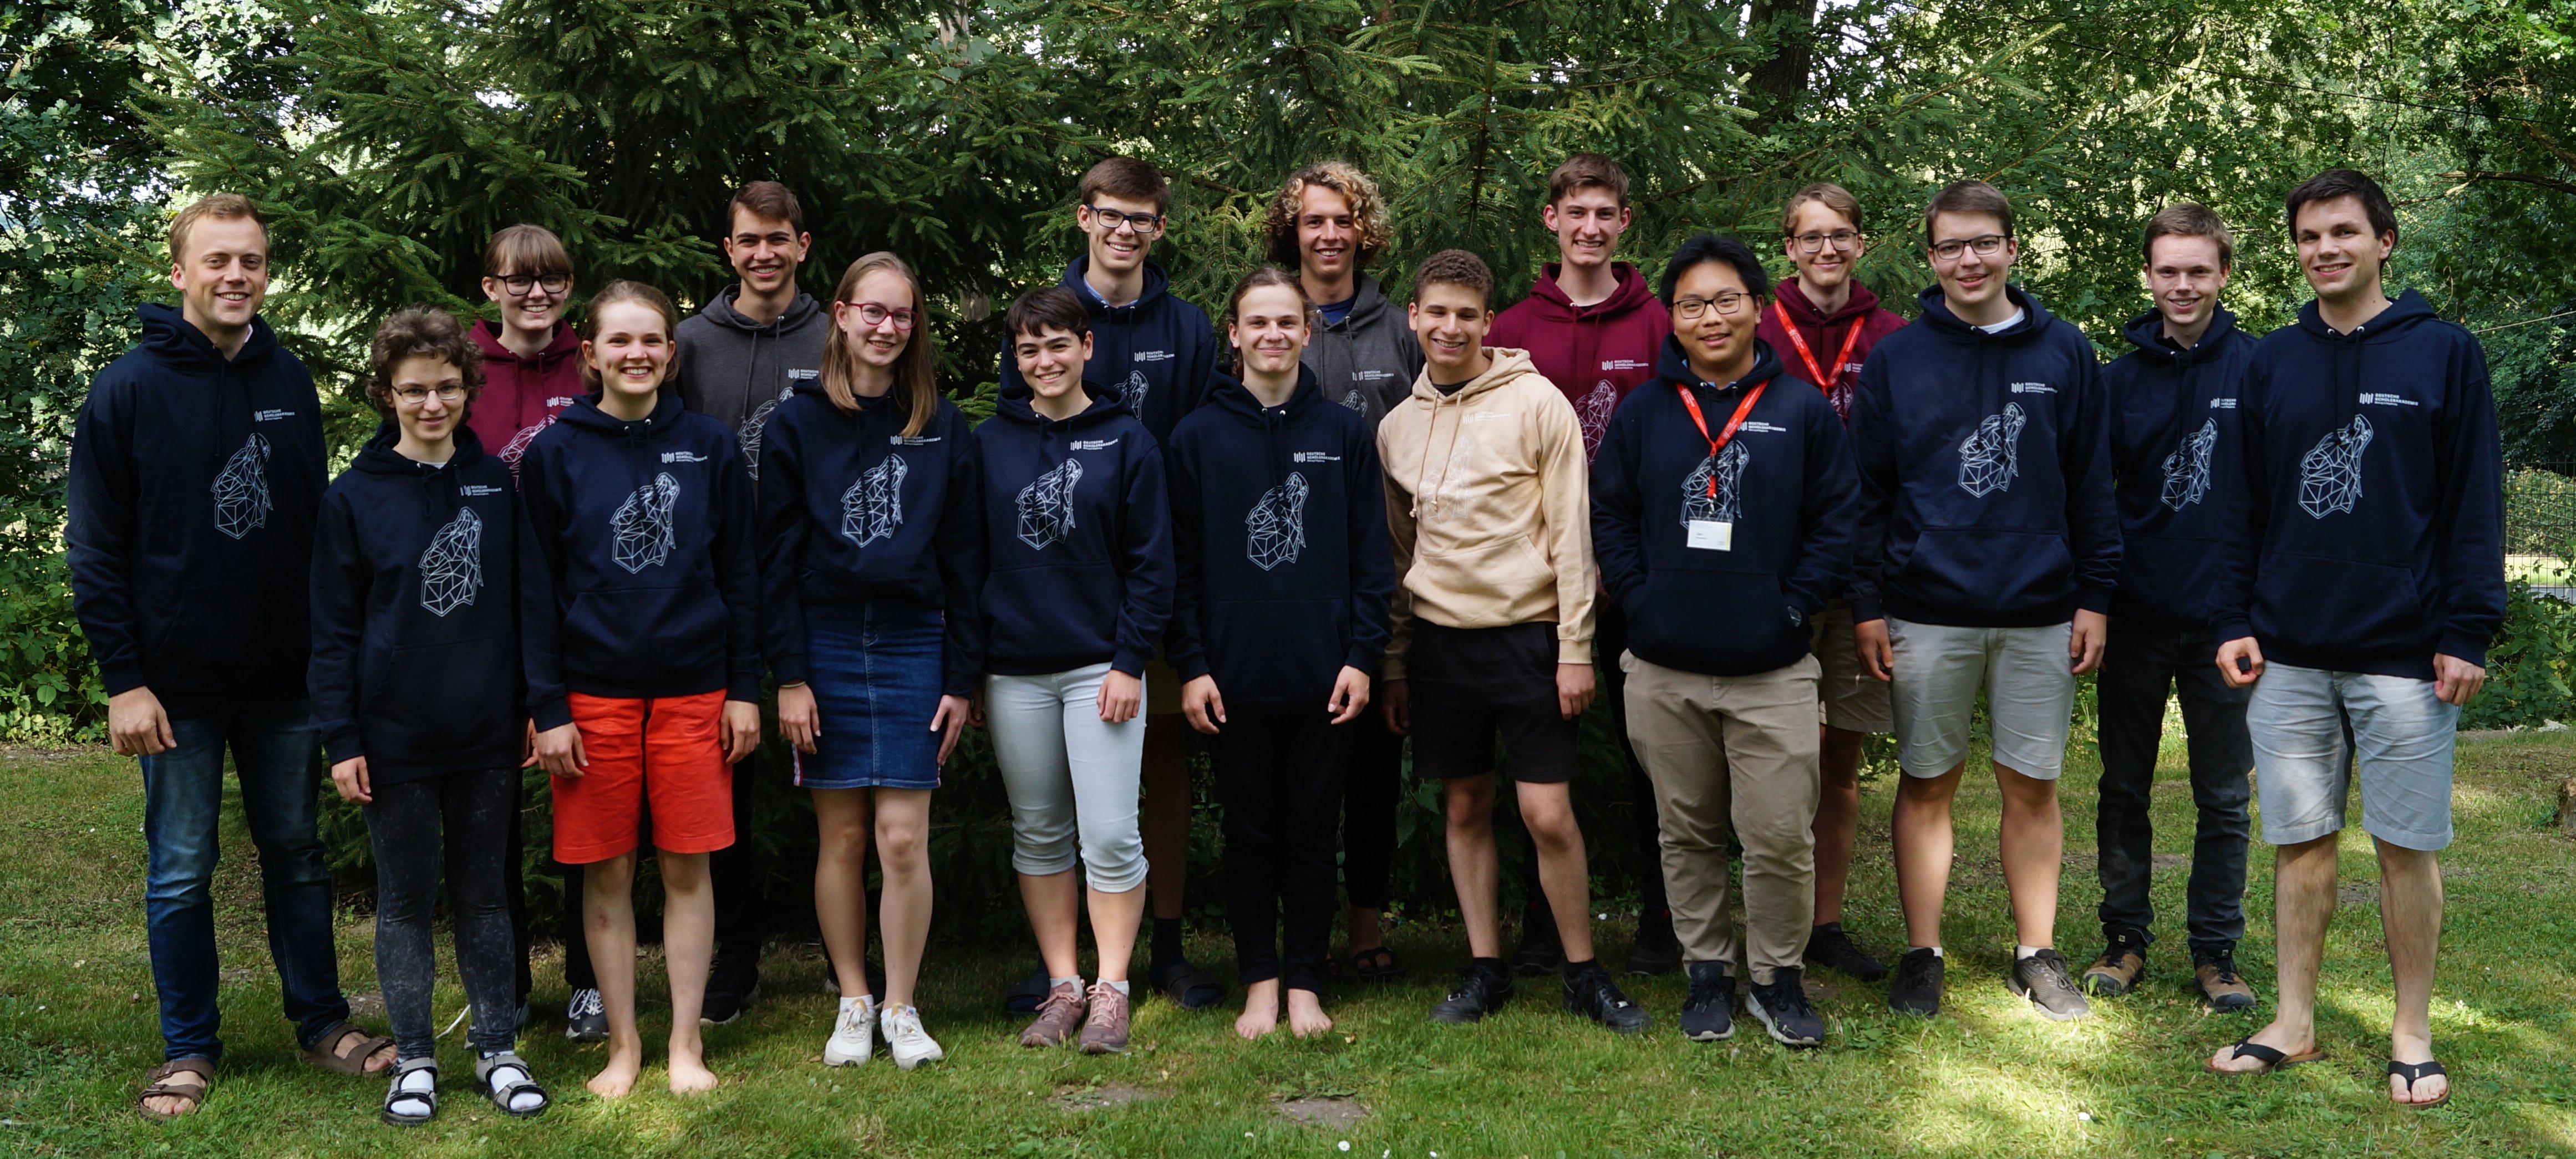
\includegraphics[width=\textwidth]{k4.2/kursfoto.jpg}
    \caption{Kursteilnehmer:innen und Kursleiter}
\end{figure}

Information ist ein allgegenwärtiger Begriff. Jede:r hat ein Gefühl dafür, was es heißt Informationen zu bekommen, mehr Informationen zu haben als jemand anderes und aus Informationen zu lernen.
Informationstheorie definiert Information auf eine scharfe mathematische Art und Weise, kann alle wesentlichen Aspekte des Sprachgebrauchs abbilden und ermöglicht es darüber hinaus, Informationen in Bits zu messen.

Der Kurs führt zunächst in die Informationstheorie und die bayessche Wahrscheinlichkeitsrechnung ein.
Mithilfe dieser Sichtweise erklärt der Kurs, was es heißt durch Informationen zu lernen und was es in diesen Kontext bedeutet \enquote{optimal} zu lernen.
Als Anwendung dieser Theorie beschäftigt sich der Kurs mit bildgebenden Verfahren von wissenschaftlichen Messgeräten, wie etwa Computertomographen (CT) oder Radioteleskopen.
Anders als herkömmliche Kameras, vermessen diese Instrumente das aufzunehmende Objekt nur indirekt.

Für die meisten dieser Anwendungen ist es nicht möglich \enquote{perfekt} aus den Messdaten zu Lernen, weshalb Näherungslösungen benutzt werden müssen.
Hierfür vermittelt der Kurs Grundlagen in Linearer Algebra und Analysis.
Im Kurs erarbeiten sich die Teilnehmenden in Gruppenarbeit am Computer, solche Näherungslösungen zu berechnen.

Das Kursziel ist es, dass die Teilnehmenden selbständig ein bildgebendes Verfahren für ein Messinstrument in Python schreiben, um damit ein aus den Rohdaten eines CT-Scans oder den Radioteleskopdaten vom Schwarzen Loch M87* ein Bild zu rekonstruieren.
Im Vorfeld der Akademie soll ein Vortrag vorbereitet werden mit hierzu bereitgestellter passender Literatur.
Zusätzlich wird vorab Material zur Verfügung gestellt anhand dessen sich Teilnehmende mit der Programmiersprache Python vertraut machen sollen.


\section{Einleitung}
\sectionauthor{Natalie Teplitska, Leo Bergmann}

Unser Kurs beschäftigte sich mit der computergestützten Gewinnung von Bildern aus Rohdaten.
Bei vielen Untersuchungsobjekten in der Physik und Medizin benötigt man bildgebende Verfahren, weil Messungen nur indirekt möglich sind.
Daher erarbeiteten wir uns notwendige mathematische Konzepte der Informationstheorie (IT) und wandten diese auf ein Beispiel aus der Radioastronomie und auf Computertomografie an.

Da wir Theorien aus diversen Anwendungsbereichen benötigten, haben wir uns diese bereits vor der Akademie im mithilfe vom Postern angeeignet und innerhalb der ersten Tage den anderen vorgestellt.
Dazu hielt jede:r einen 20-minütigen Vortrag auf Grundlage des Posters innerhalb eines durchdachten Rotationssystems.
Die Poster wurden am ersten Tag aufgehängt und weckten somit das Interesse der anderen Kurse und personalisierten den Standort.

Diese Fülle an Informationen vervollständigten Gordian und Philipp mit ihrem Wissen und ihrer Erfahrung in mehreren Input-Sessions, welche vornehmlich die erste Woche in Anspruch nahmen
Wir erhielten, alternierend von Gordian und Philipp eine Einführung in die IT, Radioastronomie, Staubtomografie und ganz viel Mathematik.

\begin{figure}
    \centering
    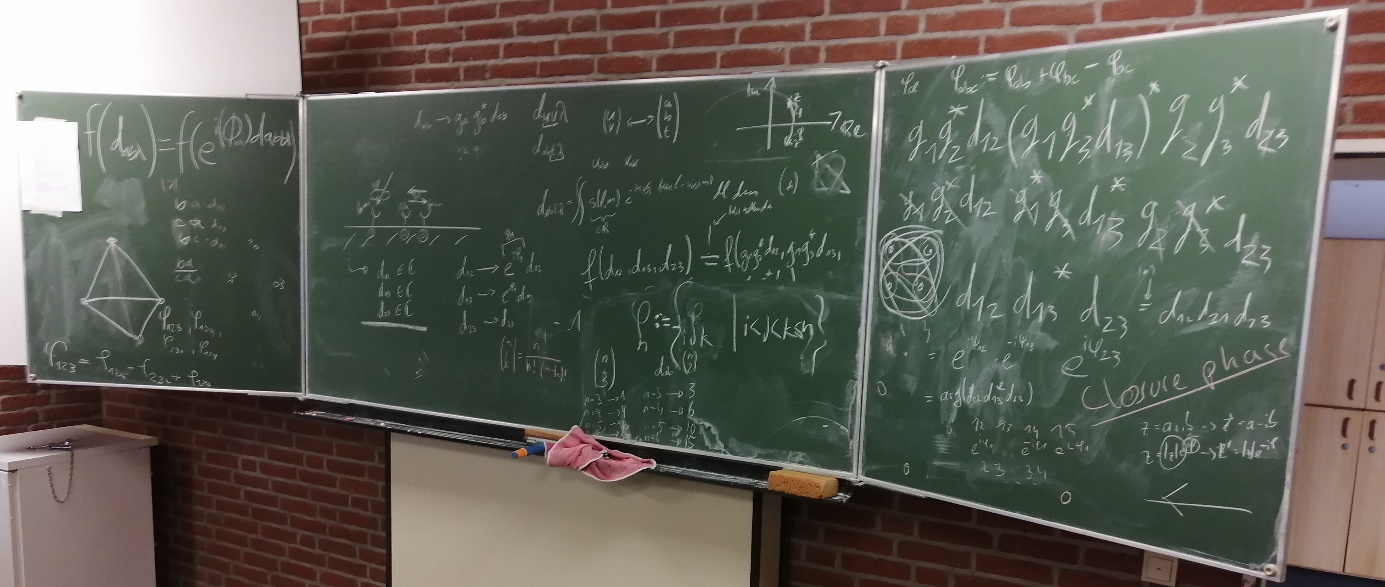
\includegraphics[width=0.8\textwidth]{k4.2/tafelbild.png}
    \caption{Tafel-Chaos}
\end{figure}


\begin{figure}
    \centering
	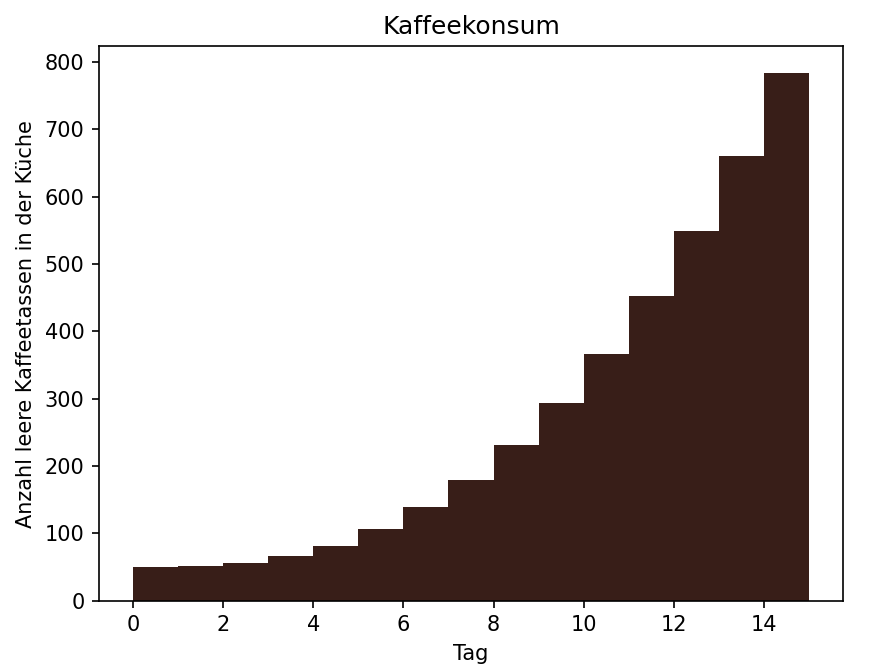
\includegraphics[width=0.5\textwidth]{k4.2/kaffee.png}
	\caption{Kaffeekonsum}
    \label{k4.2.fig.kaffee}
\end{figure}

In der zweiten Woche arbeiteten wir an eigenen Projekten.
Je zwei Projektteams beschäftigen sich mit Datenverarbeitung aus der Radioastronomie und der Computer-Tomographie.
Das fünfte Projektteam erarbeitete weitere mathematische Konzepte, welche für beide Projekte essenziell waren.
Die Projektarbeit gab uns die Möglichkeit, unser Wissen eigenständig anzuwenden.
Allerdings mussten besonders gegen Ende der Akademie Teile der Projektarbeit außerhalb der Kurse erledigt werden, was sich im allgemeinen Kaffeekonsum der Akademie niederschlug (siehe \cref{k4.2.fig.kaffee}).
Es war ein hartes Stück Arbeit, welches wir mit Python und viel Kaffee jedoch schlussendlich in den Griff bekamen.
Das Ergebnis kann sich sehen lassen!


\section{Theorem von Cox}
\sectionauthor{Patricia Hackl, Mara Germann, (Lara Müller)}
%Wie berechnet man die Wahscheinlichkeit eines Ereignisses, dem ein anderes Ereignis zu Grunde liegt? Um diese Frage zu beantworten, bedarf es der Wahrscheinlichkeitsrechnung. 
Wie wird die Wahrscheinlichkeit eines Ereignisses, dem ein anderes Ereignis zugrunde liegt, berechnet? Um diese Frage zu beantworten, bedarf es der Wahrscheinlichkeitsrechnung.

Bei dem Theorem von Cox wird die Wahrscheinlichkeitsrechnung aus der Logik hergeleitet. Im Grenzfall für absolute Sicherheit, für das Eintreten beziehungsweise Nichteintreten von Ereignissen, geht die Wahrscheinlichkeitsrechnung in wahr/falsch Aussagen und boolsche Logik über. Mit dem Theorem von Cox entsteht eine in sich konsistente (einheitliche) Theorie für die Wahrscheinlichkeitsrechnung, aus der sich herleiten lässt, dass man Wahrscheinlichkeiten als Grad der Plausibilität interpretieren kann. Es wird später deutlich werden, dass die Plausibilität der Wahrscheinlichkeit entspricht.
Das Theorem von Cox beruht auf drei Axiomen, die die Begründung der Bayes'schen Wahrscheinlichkeitsrechnung sind.


\begin{enumerate}
 \item Der \emph{Grad der Plausibilität} eines Ereignisses $B$ unter der Bedingung, dass $A$ wahr ist $\{B|A\}$, wird als reelle Zahl dargestellt. Für hohe Plausibilitäten werden hohe Zahlenwerte gewählt. Dies ermöglicht den universellen Vergleich voneinander unabhängiger Plausibilitäten.
 
 \item Sinnvolle Ergebnisse werden unter qualitativem Miteinbezug des Verstandes und durch logische Schlussfolgerungen erzielt.
 \item Es müssen alle verfügbaren Informationen miteinbezogen werden. An die Schlussfolgerungen wird die Anforderung der Konsistenz gestellt, sodass alle Sätze, die gleiches Wissen vermitteln, auf gleiche Plausibilitäten hinführen müssen.
\end{enumerate}


Aus dem Theorem von Cox lassen sich unter anderem die Summen- und Produktregel, die essentiell für die Wahrscheinlichkeitsrechnung sind, aus einfachen Axiomen herleiten.
Es verbindet die Logik mit der Wahrscheinlichkeitsrechnung. Im Folgenden sind $A$, $B$ und $C$ drei Ereignisse.

Die Produktregel beschreibt die Plausibilität $w$ der Ereignisse $B$ und $C$ unter der Bedingung, dass $A$ wahr ist $w(BC|A)$. Dies entspricht der Plausibilität des Eintretens von $B$ unter der Bedingung, dass $A$ bereits eingetreten ist $w(B|A)$, 
multipliziert mit der Plausibilität des Eintretens von $C$ unter der Bedingung, dass $AB$ wahr ist $w(C|AB)$. Als Formel ausgedrückt:

\begin{equation}
    w(\{BC|A\})=w(\{B|A\})\cdot w(\{C|AB\}) .
\end{equation}



\noindent Die Produktregel kann auf bedingte Wahrscheinlichkeiten übertragen werden:
\begin{equation}
P(B \wedge C|A) = P(B|A)\cdot P(C|AB).
\end{equation}

Dabei versteht man unter $P(B \wedge C|A)$ die Wahrscheinlichkeit für $B$ und $C$ unter der Bedingung $A$.
Aus der Produktregel folgt, dass 1 für die Wahrheit eines Ereignisses und 0 für die Unmöglichkeit eines Ereignisses steht. Dies dient als Grundlage für die Summenregel:

\begin{equation}
    w_{ges}=w(\{B|A\}) + w(\{\bar{B}|A\})= 1 .
\end{equation}

Die Gesamtplausibilität unter der Bedingung $A$ ist die Plausibilität von $B$ unter der Bedingung $A$ 
und die Plausibilität des Gegenereignisses von $B$, ebenfalls unter der Bedingung $A$. Die Summe der beiden Wahrscheinlichkeiten ist 1.


\section{Wahrscheinlichkeitstheorie}\label{k4.2.bayes}
\sectionauthor{Patricia Hackl, Mara Germann, (Natalie Teplitska)}

Die Bayes'sche Statistik beruht auf dem Rechnen mit bedingten Wahrscheinlichkeiten. Darunter versteht man die Wahrscheinlichkeit, dass ein bestimmtes Ereignis $B$ eintritt, unter der Bedingung, dass ein Ereignis $A$ bereits eingetreten ist. Diese Gleichung wird Satz von Bayes genannt:
\begin{equation}
P(B|A) = \frac{P(A \wedge B)}{P(A)} = \frac{P(B|A)\cdot P(A)}{P(B)}.
\end{equation}
%Obige Gleichung wird auch Satz von Bayes genannt. 

Bei unendlich vielen Ereignissen kann nicht jedem Ereignis eine bestimmte Wahrscheinlichkeit zugeordnet werden. Daher gibt man die Wahrscheinlichkeitsdichte an. Dabei beschreibt $x$ alle möglichen Ereignisse. Weil alle Wahrscheinlichkeiten in Summe $1$ ergeben müssen, gilt für die Fläche unter der gesamten Funktion:
\begin{equation}
\int_{- \infty }^ {+ \infty} P(x) \,\mbox{d}x = 1.
\end{equation}

Den Satz von Bayes wird verwendet, um aus Daten $d$, die aus einem Experiment gewonnen wurden, das Signal $s$ zu berechnen. Wenn $d$ eine verrauschte Tonaufnahme wäre, dann wäre $s$ das Tonsignal ohne Rauschen. Die Hintergrundinformation $I$ definiert das Modell. 


 %Die Hintergrundinformation $I$ definiert das Modell, in dem wir arbeiten. Man gewinnt durch ein Experiment die Daten $d$. Diese benötigt man um das Signal $s$ aus den Daten zu berechnen.
 % $P(s|I)$ beschreibt die Wahrscheinlichkeitsverteilung des Parameters $s$ des Modells vor der Messung.
 
 $P(s|d,I)$ gibt die Wahrscheinlichkeitsverteilung des Parameters $s$ an und wird Posterior genannt. Nach dem Satz von Bayes gilt:
 
\begin{equation}
P(s|d,I) = \frac{P(d|s,I)\cdot P(s|I)}{P(d|I)}.
\end{equation}

\begin{itemize}
 \item $P(s|I)$ gibt die Wahrscheinlichkeitsverteilung des Parameters vor dem Einbeziehen der Daten an (Prior).
 \item $P(d|I)$ ist der Normierungsparameter (Evidenz).
 \item $P(d|s,I)$ beschreibt die Wahrscheinlichkeit für die Messdaten mit gegebenem Parameter (Likelihood). \label{k4.2.likelihood}
\end{itemize}

Das Experiment kann mehrfach wiederholt werden, dabei werden neue Daten gewonnen. So dient der Posterior bei erneuter Durchführung als Prior. Wir lernen sukzessive von den neuen Daten $d$ und aktualisieren unser Wissen über Signal $s$.


\section{Normalverteilung und Kovarianz}
\sectionauthor{Patricia Hackl, Lara Müller}

Im Hinblick auf die Bayes'sche Wahrscheinlichkeitstheorie ist die Gauß'sche Normalverteilung (auch: Gauß'sche Glockenkurve) von Bedeutung.
Es lässt sich zeigen, dass die Summe von identisch verteilten und voneinander unabhängigen Zufallszahlen im Limes (Anzahl Wiederholungen $\rightarrow \infty$) zur Normalverteilung konvergiert.
Die einem Zufallsexperiment zugehörige Gauß'sche Normalverteilung ist vollständig definiert über ihren Erwartungswert $\bar{x}$ und die Kovarianz $\Sigma$:
\begin{equation}
\mathcal{G} (x - \bar{x}, \Sigma) = \displaystyle\frac{1}{\sqrt{2 \pi \Sigma}} \exp \left(- \displaystyle\frac{1}{2} \cdot (x - \bar{x}) \cdot \Sigma^{-1} \cdot (x - \bar{x}) \right).
\end{equation}
Analog zur Summenregel gilt auch für das Integral über die Normalverteilung:
\begin{equation} 
\int_{- \infty}^{\infty} \mathcal{G} (x - \bar{x}, \Sigma) dx = 1.
\end{equation}

\subsection{Erwartungswert}
Der Erwartungswert selbst ist definiert als die gewichtete Summe aus den Wahrscheinlichkeiten für die Zufallsvariable $x _i$ und bestimmt im spezifischen Fall der Normalverteilung, an welcher Stelle das Maximum auftritt (Verschiebung der Glockenkurve entlang der x-Achse). Dieser Wert muss nicht zwingend realisierbar sein. In der Formel entspricht $\chi$ dem Raum, auf dem $P(x)$ definiert ist:
\begin{equation}
\mathbb{E} _{P(x)} [x] = \int_{\chi} x P(x) dx .
\end{equation}

\subsection{Varianz und Standardabweichung}
Genauer betrachtet stellt die Kovarianz $\Sigma$ die Streuung um den Erwartungswert dar und entspricht somit der Abweichung vom Mittelwert. Diese ist immer positiv:
\begin{align}\text{Cov} [x, x] &= \mathbb{E} _{P(x)} [x \ x^{\dagger}] - \mathbb{E} _{P(x)} [x] \cdot (\mathbb{E} _{P(x)} [x])^{\dagger} 
&= \int_ {\chi} (x - \mathbb{E} _{P(x)} [x]) (x - \mathbb{E} _{P(x)} [x])^{\dagger} P(x) dx \geq 0.
\end{align}
Die Varianz ist als Diagonale der Kovarianzmatrix definiert. Die Standardabweichung $\sigma$ beschreibt das Maß der Streubreite und stellt die Wurzel der Varianz dar:
\begin{equation}
\sigma _{P(x)} [x] = \sqrt{\text{Var} _{P(x)} [x]}.
\end{equation}

Mithilfe der Gauß'schen Glockenkurve lassen sich nun vielfältige Zufallsexperimente beschreiben und entsprechende Wahrscheinlichkeitsverteilungen konstruieren. In Bezug auf den Wiener Filter wird die Normalverteilung nicht nur als Prior, sondern auch als Likelihood benötigt, um Datenlücken zu füllen, die aufgrund des Abstands der Antennen des Radioteleskops auftreten. Zudem ist das Rauschen, also die Ungenauigkeit in den Messdaten, normalverteilt und kann so aus den Daten extrahiert werden.


\section{Komplexe Zahlen}
\sectionauthor{Natalie Teplitska, Ole Fleck, Mara Germann}
Da in der Radioastronomie die Messdaten komplexe Zahlen sind, hat sich unser Kurs auch mit diesen beschäftigt.

Die Menge $\mathbb{C}$ ist die Menge aller Zahlen $z=a+b\cdot i$ für $a, b \in \mathbb{R}$. Dabei wird $a$ als Realteil und $b$ als Imaginärteil bezeichnet. Weiterhin ist $i$ die imagin\"are Einheit und definiert über die Eigenschaft: $i^{2} = -1$. Für $b = 0$ erhalten wir die bereits bekannten reellen Zahlen. Man kann $\mathbb{C}$ somit als zweidimensionalen reellen Vektorraum interpretieren.

Die komplex konjugierte von $z=a+b\cdot i$ ist definiert als $\bar{z}=a-b\cdot i$. Das Produkt aus $z$ und $\bar{z}$ hat die Eigenschaft, dass $z\cdot \bar{z}=(a+b\cdot i)\cdot (a-b\cdot i)=a^2-b\cdot i^2=a^2+b^2$ eine reelle Zahl ist.

Zwei komplexe Zahlen werden addiert, indem ihre Real- und Imaginärteile separat addiert bzw. subtrahiert werden. Auch die Multiplikation funktioniert ähnlich wie in $\mathbb{R}$, es sollte jedoch stets bedacht werden, dass $i\cdot i=-1$.Die Division von komplexen Zahlen gestaltet sich etwas komplizierter. Hier hilft es oft, mit der konjugierten komplexen Zahl des Nenners zu erweitern, sodass im Nenner kein Imaginärteil mehr vorkommt und der Ausdruck sich so erheblich vereinfacht.

Die Menge $\mathbb{C}$ lässt sich geometrisch in ein einem kartesischen Koordinatensystem darstellen, wobei die x-Achse für a und die y-Achse für b steht. Jede komplexe Zahl $z=a+b\cdot i$ entspricht dann genau einem Vektor $\begin{pmatrix} a\\b
\end{pmatrix}$.

Bisher haben wir mit den komplexen Zahlen in kartesischen Koordinaten gerechnet. Sie lassen sich aber auch als Polarform angeben:

\begin{equation}
z=r\cdot e^{i\cdot\phi}.
\end{equation}

Dabei ist $\phi$ der Winkel des Vektors zur x-Achse und r seine Länge. Bei der Multiplikation solcher Vektoren werden Winkel addiert und Längen multipliziert. Eine konjugierte komplexe Zahl ist dadurch äquivalent zur Spiegelung des Vektors an der reellen Achse.


\section{Lineare Abbildungen zwischen Vektorräumen}
\sectionauthor{Lara Müller, Chuyang Wang, Patricia Hackl}

Der folgende Abschnitt befasst sich mit den Grundlagen linearer algebraischer Berechungen und definiert in diesem Kontext lineare Abbildungen und zugehörige Vektorräume.

\subsection{Grundlagen linearer Algebra}
Ein Vektorraum über dem Körper $K$ einer Zahlenmenge ist definiert als Menge von Vektoren $V$, die einen entsprechenden Vektorraum beschreiben. Für die Vektoren $a$, $b$ und $c$ eines linearen Vektorraums müssen folgende grundlegende Rechenregeln gelten:
\begin{itemize}
\item Kommutativgesetz: $a + b = b + a$
\item Assoziativgesetz: $a + b + c = (a + b) + c = a + (b + c)$
\item Distributivgesetz: $a \cdot (b + c) = a \cdot b + a \cdot c$
\end{itemize}

Der Gegenvektor eines Vektors $a$ ist definiert als $z = -a$, sodass gilt $a + z = 0$. Eine skalare Vervielfachung bechreibt allgemein die Multiplikation eines Vektors $a$ mit einer reellen Zahl $\lambda \in \mathbb{R}$, wodurch die Vektorlänge variiert wird. Für $\lambda < 0$ wird zudem die Richtung des Vektors umgekehrt. Im Beispiel eines dreidimensionalen Vektors $a$ ergibt sich dementsprechend:
\begin{equation}
a \cdot \lambda = \left(\begin{array}{c} a_1 \\ a_2 \\ a_3 \end{array}\right)\cdot \lambda=\left(\begin{array}{c} a_3 \lambda \\ a_2 \lambda \\ a_1 \lambda \end{array}\right)
\end{equation}

\subsection{Lineare Abbildungen}
Als lineare Abbildung wird jede Abbildung definiert, deren Additivität ($f(v + w) = f(v) + f(w)$ für alle $v$, $w \in V$) und Homogenität ($f(\lambda v) = \lambda f(v)$ für alle $\lambda \in K$, $v \in V$) gegeben sind. Bezüglich der zwei $K$-Vektorräume $V$ und $W$ ist die Abbildung $f: V \rightarrow W$ linear, sofern gilt:
\begin{equation}
f(\lambda v + \mu w)=\lambda f(v) + \mu f(w) \quad \forall \; \lambda, \mu \in K \quad \forall \; v, w \in V.
\end{equation}

\subsection{Eigenschaften von Vektorräumen}
Darüber hinaus bezeichnet man die Menge der Vektoren, die auf den Nullvektor $\vec{o}$ abgebildet werden, als Kern der zugehörigen linearen Abbildung. Der Kern $\mathrm{ker}(f):= \{v \in V \; \big\vert \; f(v) = 0 \}$ entspricht demnach einem Vektor aus dem Vektorraum $V$ ($\mathrm{ker}(f) \subseteq V$), in dem auch der Nullvektor enthalten ist ($0 \in \mathrm{ker}(f)$). Vektorräume können unendlichdimensonal sein und somit beispielsweise als reeller ($V \in \mathbb{R}^{n}$) oder komplexer ($V \in \mathbb{C}^{n}$) Vektorraum auftreten. Die jeweilige Dimension eines endlichdimensionalen Vektorraums $K^n$ kann über die zur Darstellung zwingend notwendige Mindestanzahl $n$ an Basisvektoren bestimmt werden. Diese sind so definiert, dass sich jeder andere Vektor $c$ über Linearkombinationen der Basisvektoren $b_i$ beschreiben lässt:
\begin{equation}
c = \sum_i^{n} \alpha_i b_i.
\end{equation}

\subsection{Darstellung linearer Abbildungen durch Matrizen}
Lineare Abbildungen lassen sich auch über Matrizen darstellen. Beispielsweise gilt für eine lineare Abbildung in dem zweidimensionalen Vektorraum $K^{n}$, der über die Basisvektoren $\vec{u}$ und $\vec{v}$ dargestellt werden kann:
\begin{equation}x \cdot \left(\begin{array}{c} u_1 \\ u_2 \end{array}\right) + y \cdot \left(\begin{array}{c} v_1 \\ v_2 \end{array}\right) = \left(\begin{array}{c} u_1 x + v_1 y \\ u_2 x + v_2 y \end{array}\right) = \left( \begin{array}{rr} u_1 & v_1 \\ u_2 & v_2 \end{array}\right) \cdot \left(\begin{array}{c} x \\ y \end{array}\right)
\end{equation}

Die resultierende $2$x$2$-Matrix beinhaltet entsprechend der Matrix-Spalten sowohl das Bild des ersten, als auch das des zweiten Basisvektors. Allgemein lassen sich lineare Abbildungen $f(\vec{x})$ über eine zugehörige Matrix $A$ darstellen:
\begin{equation}
f(\vec{x}) = A \cdot \vec{x}.
\end{equation}

Bei einer linearen Abbildung stellt $f(\vec{x})$ selbst auch stets wieder einen Vektor dar. Dabei bleiben Streckenverhältnisse und Lagebeziehungen der Vektoren zueinander unverändert. Im Gegensatz zur Drehung, Scherung und Projektion sind Krümmungen bei einer linearen Abbildung nicht möglich. Daher werden diese Abbildungen auch als strukturerhaltende Abbildungen zwischen Vektorräumen bezeichnet.

\subsection{Matrix-Vektor-Multiplikation}
\label{k4.2.linalg}
Das Vektor-Matrix-Produkt wird für die Matrix $A \in \mathbb{R}^{N \times M}$ und den Vektor $x \in \mathbb{R}^M$ wie folgt definiert:

\begin{equation}
  \begin{aligned}
    Ax &= \begin{pmatrix}
      a_{11} & a_{12} & ... & a_{1M} \\ 
      a_{21} & a_{22} & ... & a_{2M} \\ 
      ... & ... & ... & ... \\ 
      a_{N1} & a_{N2} & ... & a_{NM} \\ 
    \end{pmatrix}
    \cdot 
    \begin{pmatrix}
      x_1 \\ x_2 \\ ... \\ x_M
    \end{pmatrix} \\[2ex]
    &=  \begin{pmatrix}
      a_{11}x_1 + a_{12}x_2 +... + a_{1M}x_M \\ 
      a_{21}x_1 + a_{22}x_2 + ... + a_{2M}x_M \\ 
      ... + ... + ... + ... \\ 
      a_{N1}x_1 + a_{N2}x_2 + ... + a_{NM}x_M \\ 
    \end{pmatrix}
  \end{aligned}
\end{equation}

Dabei wird jede Zeile der Matrix mit dem Vektor elementweise multipliziert. Die Summe der Produkte bildet die Komponente des resultierenden Vektors.


\section{Eigenwertproblem}
\sectionauthor{Lara Müller, Chuyang Wang, Benjamin Knöbel del Olmo}

\subsection{Definitionen}\label{k4.2.eigen.def}

Die Eigenvektoren einer Matrix sind diejenigen Vektoren, welche nach Anwendung dieser Matrix immer auf einem Vielfachen von sich selbst liegen.
Formal werden die Eigenvektoren einer quadratischen Matrix $A \in \mathbb{R}^{x \times x}$ definiert als $v \in \mathbb{R}^{x}, v \neq 0$, sodass $A \cdot v = \lambda \cdot v$ erfüllt ist. Man nennt das Skalar $\lambda$ den zu $v$ zugehörigen Eigenwert.

Durch Äquivalenzumformung erhält man

\begin{equation}
  \label{k4.2.eigen.def.lgs}
  \begin{aligned}
     &                 & A \cdot v               & = \lambda \cdot v   &                                 & \\
     & \Leftrightarrow & A \cdot v               & = \lambda E \cdot v & \text{mit } v = Ev              & \\
     & \Leftrightarrow & (A - \lambda E) \cdot v & = 0                 &                                 & \\
     & \Leftrightarrow & Bx                      & = 0  \quad \quad    & \text{mit } B = (A - \lambda E) & \\
  \end{aligned}
\end{equation}

Die \emph{Determinante} einer Matrix ist ein skalarer Wert, welcher die Lösbarkeit dieser Matrix beschreibt. Dieses lineare Gleichungssystem aus \cref{k4.2.eigen.def.lgs} hat genau dann nicht-triviale Lösungen ($x \neq 0$), wenn die Determinante von $B$ gleich $0$ ist. Also gilt $\det (B) = \det (A - \lambda E) = 0$.

Bei dem Eigenwertproblem gilt es, diese Vektoren sowie die zugehörigen Eigenwerte zu finden.


\subsection{Das charakteristische Polynom}

Im Allgemeinen wird das charakteristische Polynom der Matrix $A$ definiert als $\chi_A (\lambda) = \det(A - \lambda E)$. Aus \cref{k4.2.eigen.def} folgt, dass man die Nullstellen dieses Polynoms finden muss, um den Eigenwert zu berechnen.

Betrachtet man nun beispielsweise das Problem in 2D und sei $A = \begin{pmatrix}
    a & b \\
    c & d
  \end{pmatrix}$, so gilt

\begin{equation}
  \label{k4.2.eigen.charac.2d}
  \begin{aligned}
    0
     & = \chi_A (\lambda)                              \\
     & = \det(A - \lambda E)                           \\
     & = \det \begin{pmatrix}
                a - \lambda & b         \\
                c           & d-\lambda
              \end{pmatrix}                  \\
     & = (a - \lambda) \cdot (d - \lambda) - c \cdot b
  \end{aligned}
\end{equation}

Eine allgemeine Lösung für \cref{k4.2.eigen.charac.2d} kann dann mithilfe der pq-Formel berechnet werden:

\begin{equation}
  \begin{aligned}
    \lambda = \frac{a+d}{2} \pm \sqrt{\Big(\frac{(a+d)}{2}\Big)^2-ad+cb}
  \end{aligned}
\end{equation}


\subsection{Power Iteration}\label{k4.2.eigen.powerit}

Für $2 \times 2$ Matrizen lässt sich das Eigenwertproblem relativ gut lösen, da eine allgemeine Formel (vgl. pq-Formel / abc-Formel) für das charakteristische Polynom existiert. Ab dem 5. Grad ist es jedoch unmöglich, eine allgemeine Formel herzuleiten \parencite{k4.2.ramond}. % Abel Ruffini Theorem
Mit dem Power-Iteration-Algorithmus versucht man, eine Annäherung an den höchsten Eigenwert zu berechnen. Der iterative Algorithmus wählt am Anfang einen willkürlichen Wert für $b_0 \in \mathbb{R}^n$. Bei jeder Iteration aktualisiert man diesen Vektor $b$ wie folgt:

\begin{equation}
  \begin{aligned}
    b_{k+1} = \frac{Ab_k}{\left\lVert Ab_k \right\rVert }
  \end{aligned}
\end{equation}

Nach ausreichenden Iterationen kann man den größten Eigenwert $\lambda$ berechnen, indem man die Gleichung $B b_{k} = \lambda b_{k}$ nach $\lambda$ auflöst.

\subsection{Anwendungen}

Eigenwerte und Eigenvektoren sind wichtig in der Mathematik. Ein Beispiel dafür ist die Drehung durch eine Matrix: Wenn die Matrix $A$ eine Drehung um einen bestimmten Winkel beschreibt, dann ist der Eigenvektor die Drehachse, da seine Richtung durch die Drehung nicht verändert wird.


\section{Gradient Descent}

\sectionauthor{ Leo Bergmann, Benjamin Knöbel del Olmo, Cedric Balzer}



Wie in der Betrachtung von eindimensionalen Funktionen, werden für die Bestimmung der Extrema auch bei mehrdimensionalen Funktionen Ableitungen eingesetzt. Diese werden nicht mehr durch reelle Zahlen, sondern durch Vektoren ausgedrückt. Gegeben sei eine differenzierbare und konvexe Funktion $ f:\mathbb{R}^n \rightarrow \mathbb{R}, x \mapsto f(x). $ Die Ableitung von f an einem Punkt entspricht einem N-Dimensionalen Vektor. Diese Vektor wird Gradient genannt und seine Spitze zeigt immer in Richtung des stärksten Anstiegs, wobei dessen Länge der Steigung entspricht.

Der darauf basierende Gradient Descent Algorithmus wird verwendet, um das Minimum einer Fuktion zu approximieren. Dies wird durch einen iterativen Ansatz erreicht: An einem zufällig gewählten Startpunkt wird zunächst der Gradient ermittelt. Danach wird als neuen Startpunkt derjenige definiert, der durch das Gehen in die entgegengesetzte Richtung des Gradienten erreicht wird. Die Länge des gegangenen Schrittes hängt von der Länge des Gradienten ab, die durch eine Konstante, die Learning Rate, skaliert wird. Dies ermöglicht eine freie Adjustierung der Schrittgrößen, um das Minimum genauer zu treffen. Der Algorithmus endet, wenn die davor definierte, maximale Anzahl an Durchläufen erreicht, oder wenn die Schrittlänge kleiner als eine davor definierte Toleranz ist. Der Gradient Descent ist also ein Näherungs-/Optimierungsalgorithmus.



Vorausgesetzt wird, dass die Funktion differenzierbar und konvex ist, das heißt das die Verbindungslinie zwischen zwei Punkten des Graphens immer über dem Graphen liegt. Auch Funktionen mit Sattelpunkt oder die Wahl einer unpassenden Learning Rate bei der Implementierung können zu falschen Ergebnissen und langen Laufzeiten führen. Das liegt daran, dass bei zu großen Learning Rates das Minimum einfach übergangen wird, während bei zu kleinen Learning Rates der Algorithmus in lokalen Minima „stecken“ bleibt, wobei das Programm dann ohne wesentliche numerische Verbesserung weiterläuft.


\section{Conjugate Gradient}
\sectionauthor{Benjamin Knöbel del Olmo, Leo Bergmann, Chuyang Wang}

Um lineare Gleichungssysteme (LGS) effizient und exakt zu lösen, wird Conjugate Gradient verwendet, welcher auch auf der Minimabestimmung basiert.


Die Formel $Ax = b$ lässt sich auf ein LGS anwenden, wobei A eine $ n \times n $-Matrix (invariant unter Transposition) und $ b,x $ Vektoren sind. Eine quadratische Funktion $ f(x) = \frac{1}{2}xAx-bx+c $ wird definiert, (mit selben A,b und x), dessen komponentenweise Ableitung genau dann null ist, wenn das ursprüngliche LGS nach x gelöst ist, da gilt: $f'(x) = Ax-b = 0$. Daher ist das Optimieren der dem LGS entsprechenden Funktion äquivalent zum Lösen ebenjenes.


Der Algorithmus funktioniert folgendermaßen: Conjugate Gradient läuft das Residuum (der dem Gradienten entgegengesetzte Vektor, $ r = b-Ax $) ab, aber korrigiert die „Abstiegsrichtung“ unter Betrachtung aller vorher gegangenen Residuen so, dass die Abstiegsrichtung A-orthogonal (engl. conjugate, def.: $x^{T}Ay = 0$, x,y A-orthogonal) zu allen vorherigen Residuen ist. Daraus folgt, dass wir nach maximal $n$-Schritten am Ziel ankommen, da wir dann alle $n$ Dimensionen der $ n \times n $-Matrix optimal abgegangen sind. Der Algorithmus ist durch zwei Abbruchbedingungen definiert, zum einen, wenn $n$ Iterationen erreicht sind, zum andern wenn die Differenz zum Endergebnis, also dasss $ f'(x) = 0 $ gilt, klein genug ist.

Gradient Descent und Conjugate Gradient ermöglicht es uns also, lineare Gleichungssysteme zu lösen und dadurch Daten, die in Matrizen gespeichert sind, weiterzuverarbeiten. Ein Beispiel wäre die Lösung der Gleichung $ D^{-1} m = j $, auf die im Kapitel \enquote{Wiener Filter} \cref{k4.2.wiener.filter} eingegangen wird.


\section{Programmierparadigmen}
\sectionauthor{Alexander Gitnik, Clemens Ljungh, Jonas Fiedler, Aaron Gschwendt}

\subsection{Objektorientierte Programmierung}
Die objektorientierte Programmierung ist eins der am weitesten verbreiteten Programmierparadigmen. Beim objektorientierten Programmieren ist das ausschlaggebende Kriterium, dass man den Code zu sinnvollen Strukturen zusammenfasst. Dafür erstellt man Klassen, welche oftmals reale Objekte repräsentieren. 

Eine Klasse ist eine allgemeine Vorlage, aus der einzelne Objekte, die \emph{Klasseninstanzen}, initialisiert werden können. Diese Klassen besitzen zum einen Eigenschaften, \emph{Attribute} genannt, und zum anderen Handlungsmöglichkeiten, welche \emph{Methoden} genannt werden. Jede Klasse besitzt einen Konstruktor, welcher bei der Erstellung einer \emph{Instanz} der Klasse aufgerufen wird. Zudem werden gegebenenfalls die zum Erstellen einer Klasse benötigten Parameter übergeben. Objekte werden durch Zuweisung des Konstruktoraufrufs, der jeweiligen Klasse, an eine Variable initialisiert, welche nun zu einem Objekt des Klassentyps wird. Wenn sich Klassen ähneln, können gleiche \emph{Attribute} und \emph{Methoden} in einer \emph{Superklasse} definiert werden. Diese vererben den Klasseninhalt an die \emph{Unterklassen}, welche die Merkmale übernehmen.

Typischerweise werden \emph{Attribute} lediglich über \emph{Getter-} und \emph{Setter-Methoden} abgefragt und verändert, damit der Zustand des Objekts immer nur kontrolliert verändert werden kann. Dies hat den Grund, dass man nicht versehentlich einen Fehler in den inneren Zustand des Objekts einbauen möchte. Eine \emph{Setter-Methode}, kann überprüfen, welche Werte ein Attribut annimmt. Um eine Methode aufrufen zu können ist es im Normalfall nötig dies über eine bereits initialisierte Instanz der Klasse zu tun. Ein spezieller Dekorator macht die Methode statisch, was bedeutet, dass die Methode über die Klasse aufgerufen werden kann. Dies hat den Vorteil, dass man nicht erst ein Objekt initialisieren muss un die Methode nutzen zu können.

\subsection{Funktionale Programmierung}
Die funktionale Programmierung ist ein gänzlich anderes Konzept als die objektorientierte Programmierung. Funktionale Programmierung hat ihren Ursprung im Lambda-Kalkül. Das Lambda-Kalkül ist eine formale Sprache, um logische Systeme darzustellen. Es ist Turing-vollständig, dies bedeutet, dass man jedes Programm damit ausdrücken kann.

Anders als bei der objektorientierten Programmierung werden Daten bei der funktionalen Programmierung nicht in Objekten gespeichert, sondern ausschließlich durch einzelne Funktionen verarbeitet. Diese Funktionen müssen dabei \emph{pur} sein. \emph{Pure Funktionen} definieren sich dadurch, dass sie bei gleicher Eingabe immer die gleiche Ausgabe geben, da sie keinen inneren Zustand haben, welcher die Eingabe verändern könnte. Weiterhin ändern die puren Funktionen auch nichts außerhalb der eigenen Funktion.

Funktionen können als Parameter den Rückgabewert einer anderen Funktion nehmen, sodass jene ineinander verschachtelt werden. So entsteht in der funktionalen Programmierung natürlicherweise eine Kette aus verschachtelten Befehlen. Häufig wird in der funktionalen Programmierung \emph{Rekursion} verwendet, also Funktionen, die sich selbst aufrufen.

Daten sind bei der objektorientierten Programmierung zwar besser strukturiert, aber dafür sind gerade die puren Funktionen der funktionalen Programmierung einfacher für Entwickler zu verstehen, da die puren Funktionen keinen möglicherweise komplizierten inneren Zustand haben. Wichtig für die funktionale Programmierung ist das Konzept der \emph{Lazy Evaluations}. Dies bedeutet, dass Ausdrücke, erst dann ausgerechnet werden, wenn sie für ein Ergebnis benötigt werden. Dadurch kann in manchen Fällen die Laufzeit eines Programmes verringert werden, was vorteilhaft ist.

Für unsere Kursarbeit verwenden wir oft funktionale Programmierung, da wir Datensätze und probabilistische Modelle rein mathematisch verarbeiten. Außerdem ist Python gut für die funktionale Programmierung geeignet.

\subsection{Gegenüberstellung}
Insgesamt unterscheidet sich damit die objektorientierte Programmierung von der funktionalen Programmierung bereits in ihrem Ansatz. Sie ist realtitätsbezogen, wohingegen die funktionalen Programmierung lediglich an der Programmeffektivität orientiert ist. Die Umsetzung ist daher sehr verschieden, sodass in der objektorientierten Programmierung Klassen und globale Variablen gefordert werden, während die funktionale Programmierung ebendiese verbietet, und mittels puren Funktionen den Code in kleinstmögliche und unabhängige Abschnitte unterteilt.


\section{NumPy}\label{k4.2.ch.NumPy}
\sectionauthor{Cedric Balzer, Leo Bergmann}

Numerisches Python (kurz NumPy) ist eine in der Programmiersprache C geschriebene Libary für Python. Sie ermöglicht das effiziente Rechnen mit Matrizen, mehrdimensionalen Arrays und Vektoren in Python.

NumPy ist eine open-source Library, welche auf den früheren Python-Modulen Numeric und Numarray basiert. Da Python nicht für numerische Rechnung optimiert ist, greift NumPy auf C-Code zurück. Eine der Kernfunktionalitäten von NumPy ist das sogenannte \lsin{np.ndarray()}, das ein beliebig-dimensionales Array repräsentiert. Im Gegensatz zu Python-Listen müssen alle im Array gespeicherten Elemente vom selben Datentyp sein, zudem ist die Größe eines NumPy-Arrays statisch. Dies ermöglicht im Vergleich zu Listen eine schnellere Handhabung.

NumPy ist nicht im Python3-Standard enthalten und muss daher separat installiert werden:

\begin{lstlisting}
pip install numpy
\end{lstlisting}

Möchte man ein Array aus einer Liste erstellen, bietet sich folgender Code an:

\begin{lstlisting}[language=python]
>>> import numpy as np
>>> a = np.array([1, 2, 3, 4, 5])
>>> a
array([1, 2, 3, 4, 5])
\end{lstlisting}

Besteht eine übergebene Liste aus mehreren Teillisten wird ein mehrdimensionales Array erstellt:

\begin{lstlisting}[language=python]
>>> m1 = np.array([[1, 2, 3], [4, 5, 6], [7, 8, 9]])
>>> m1
array([[1,2,3],
       [4,5,6],
       [7,8,9]])
\end{lstlisting}

Möchte man auf ein Element eines eindimensionalen Arrays zugreifen, so funktioniert dies wie bei Listen. Um in mehrdimensionalen NumPy-Arrays Werte zu selektieren, wird folgende Syntax verwendet:

\begin{lstlisting}[language=python]
>>> m1[0, 0], m1[2, -1]
1, 9
\end{lstlisting}

Auf Arrays können elementweise Rechenoperatoren, wie Plus und Minus, angewandt werden. Es werden stets neue Arrays erzeugt und die Original-Arrays bleiben unverändert.

\begin{lstlisting}[language=python]
>>> r = np.arange(10)
>>> r
array([0, 1, 2, 3, 4, 5, 6, 7, 8, 9])
>>> r+1
array([1, 2, 3, 4, 5, 6, 7, 8, 9, 10])
>>> r**2
array([0, 1, 4, 9, 16, 25, 36, 49, 64, 81])
\end{lstlisting}

Des Weiteren sind in NumPy spezielle Operationen für Matrizen und Vektoren implementiert. Beispielsweise können mit \verb|np.dot()|, \verb|np.inner()| und \verb|np.outer()| Multiplikationen von Matrizen beziehungsweise Vektoren durchgeführt werden (siehe \cref{k4.2.linalg} für eine mathematische Beschreibung).

\begin{lstlisting}[language=python]
>>> np.dot([[1, 0], [0, 1]], [[4, 1], [2, 2]])
array([[4, 1],
       [2, 2]])
\end{lstlisting}

Neben \verb|np.dot()| liefert NumPy den Operator \verb|@| (und alternativ \verb|np.matmul()|), welcher ebenfalls Arrays und Matrizen multipliziert.
Bei einer Multiplikation von Vektoren und 2D Matrizen erzeugen diese Funktionen identischen Output:

\begin{itemize}
    \item Skalarmultiplikation zweier Vektoren

        \begin{lstlisting}[language=python]
>>> a = np.array([1, 2])
>>> b = np.array([2, 2])
>>> np.dot(a, b)
6
>>> a @ b
6
\end{lstlisting}

  \item Multiplikation zweier Matrizen

        \begin{lstlisting}[language=python]
>>> a = np.array([[1, 2],[5, 3]])
>>> b = np.array([[2, 2],[8, 1]])
>>> np.dot(a, b)
array([[18  4]
       [34 13]])
>>> a @ b
array([[18  4]
       [34 13]])
\end{lstlisting}

\end{itemize}

NumPy ist also die Standardbibliothek für effiziente Matrix-Vektor-Rechnung in Python. Sie liefert die Grundlagen für viele wissenschaftliche Arbeiten, so auch für unser Projekt, um Bayes'sche Bildgebungsalgorithmen zu implementieren.


\section{Pytest}
\sectionauthor{Finja Hoffmann, Alexander Gitnik}
Pytest ist ein Testing-Framework für Python, mit welchem sich die Fehlerbehebung und allgemeine Testphase in der Softwareentwicklung automatisieren lässt. Anstatt sich immer mal wieder an ausgewählten Stellen Werte ausgeben zu lassen und diese manuell zu überprüfen, kann man Test-Methoden schreiben, um so automatisiert Fehler zu erkennen. Pytest überprüft mit synthetischen Eingaben die zu testende Funktion und vergleicht die Ausgabe mit dem eingegebenen Erwartungswert.

Das Überprüfen implementiert man durch:
\begin{lstlisting}[language=python]
assert f(A) == B
\end{lstlisting}
Hierbei wird die Funktion \texttt{f} mit Eingabe \texttt{A} und Erwartungswert \texttt{B} getestet.

In einem konkreten Beispiel addiert eine Funktion den eingegebenen Wert mit \texttt{2}. Hier wird \texttt{1} eingegeben und der Erwartungswert ist \texttt{3}:
\begin{lstlisting}[language=python]
assert add_2(1) == 3
\end{lstlisting}

Pytest führt nun die zu testende Methode mit den eingegebenen Werten aus. Durch das \texttt{assert}-statement wird automatisch die Ausgabe überprüft. Sollte die erwartete Ausgabe nicht mit der tatsächlichen Ausgabe übereinstimmen wird eine Fehlermeldung angezeigt. Es wird zudem angezeigt, welche Eingabe und Code-Zeile zur Fehlermeldung geführt haben.

Die zu testende Methode beginnt mit \texttt{test\_}.

Mit dem Dekorator \texttt{@pytest.fixture} vor einer Funktion lässt sich die Eingabe von zu testenden Methoden global definieren und dessen Spezifikationen automatisieren.

Auch kann man Parameter eingeben, bei denen man eine Fehlermeldung erwartet. Es wird überprüft, ob nicht erwartete Eingaben wirklich als Fehler erkannt werden. Dafür gibt es den Befehl
\begin{lstlisting}[language=python]
import pytest
with pytest.raises({FehlerTyp}):
    pass
\end{lstlisting}
mit dem überprüft wird, ob die Funktion wirklich die erwartete Fehlermeldung zurückgibt.

Weiterhin kann man Funktionen mit einer Test-Methode durch den Dekorator
\begin{lstlisting}[language=python]
@pytest.mark.parametrize({Eingabe})
\end{lstlisting}
kennzeichnen. In diesem Fall werden die Ein- und Ausgabewerte paarweise in Klammern untereinandergeschrieben.

Wenn die automatisierten Test-Methoden ohne Fehlermeldung durchlaufen, so ist der Algorithmus scheinbar fehlerfrei. Dabei können Fehler aber nicht vollständig ausgeschlossen werden, da die Testung immer nur so gut ist wie die Ideen-Vielfalt zu potenziellen Fehlerquellen. Nicht bekannte, ungetestete Fehler können nicht vermieden werden.


\section{Git}
\sectionauthor{Jonas Fiedler, Clemens Ljungh}

Mit der Versionsmanagement-Software Git kann Kooperation zwischen mehreren Programmierern ermöglicht werden. Git beschäftigt sich hauptsächlich mit dem Verwalten von Versionen des Codes und der Zusammenführung von Code Änderungen. Dafür erstellt Git einen Versionsverlauf, welcher es ermöglicht, Versionen des Codes zurückrollen um Bugs zu identifizieren und das Nachverfolgen von Code-Änderungen von wichtigen Updates zu ermöglichen. Dabei wird zwischen lokaler Dateispeicherung und Speicherung im serverseitigen Bereich unterschieden. Der Server ermöglicht den Nutzern, Code herunterzuladen, ihn zu bearbeiten und letztendlich in überarbeiteter Version wieder an den Server zu übermitteln, wo dieser dann mit anderen Nutzern ausgetauscht werden kann.

Generell ist es in Git möglich verschiedene Versionsstränge (Branches) aufzubauen. Diese Branches ermöglichen die Modifikation an verschiedenen Bereichen und ein strukturierte Entwicklung von Features. In diesen Branches können somit bspw. Bugs unabhängig gelöst werden und neue Funktionen getestet sowie implementiert werden. Sobald diese ordnungsgemäß funktionieren, werden sie auf den nächst höheren Branch, eine in der Hierarchie übergeordnete Ebene, geschoben (Merge) und somit mit dem Rest des Codes wieder vereint.

In Git gibt es verschiedene Stadien, der \enquote{Codeverarbeitung} um eine Codeversion zu speichern. Dabei beschreibt \verb|git add| den Vorgang wo die Datei von dem Working-Directory (lokal), in die Staging Area (auch lokal) verschoben wird. Der wichtigste Befehl in Git ist \verb|git commit|, dieser hält den aktuellen Zustand des gesamten Projektes fest und speichert diesen im Localrepo. Danach ermöglicht \verb|git push| das Übertragen des Codes an den Server. Der umgekehrte Schritt dazu ist \verb|git pull|. Dies lädt die aktuellste Version des Projektes vom Remoterepo in das Localrepo des Users.

Aufgrund der diversen Verwaltungsoptionen und der Möglichkeit kollaborativ in Git zu arbeiten, wird dieses Tool von vielen Software-Developern, sowie Unternehmen verwendet.


\section{Radioastronomie}
\sectionauthor{Constantin Burmeister, (Ole Fleck)}

Radioastronomie dient der Beobachtung von astrophysikalischen Prozessen, die Radiowellen, also Wellen langer Wellenlänge, aussenden. Um hohe Auflösungen zu erreichen, werden Radiointerferometer verwendet, welche Signale mehrerer Antennen so zusammenfügen, als würde es sich um eine Antenne handeln.

Allgemein ist der minimal auflösbare Bildwinkel $\delta\theta$ eines Teleskops abhängig von der Wellenlänge $\lambda$, des beobachteten Lichts, und dem Spiegeldurchmesser $D$ des Teleskops mit \begin{eqnarray} \label{k4.2.radioformel}
\delta\theta\approx1.22\frac{\lambda}{D}.
\end{eqnarray}
Da die Radioastronomie große Wellenlängen verwendet, sind hier auch bei Teleskopen mit großen Spiegeldurchmessern von über $100\text{m}$ nur geringe Auflösungen möglich.

\begin{figure}[htb]
\centering
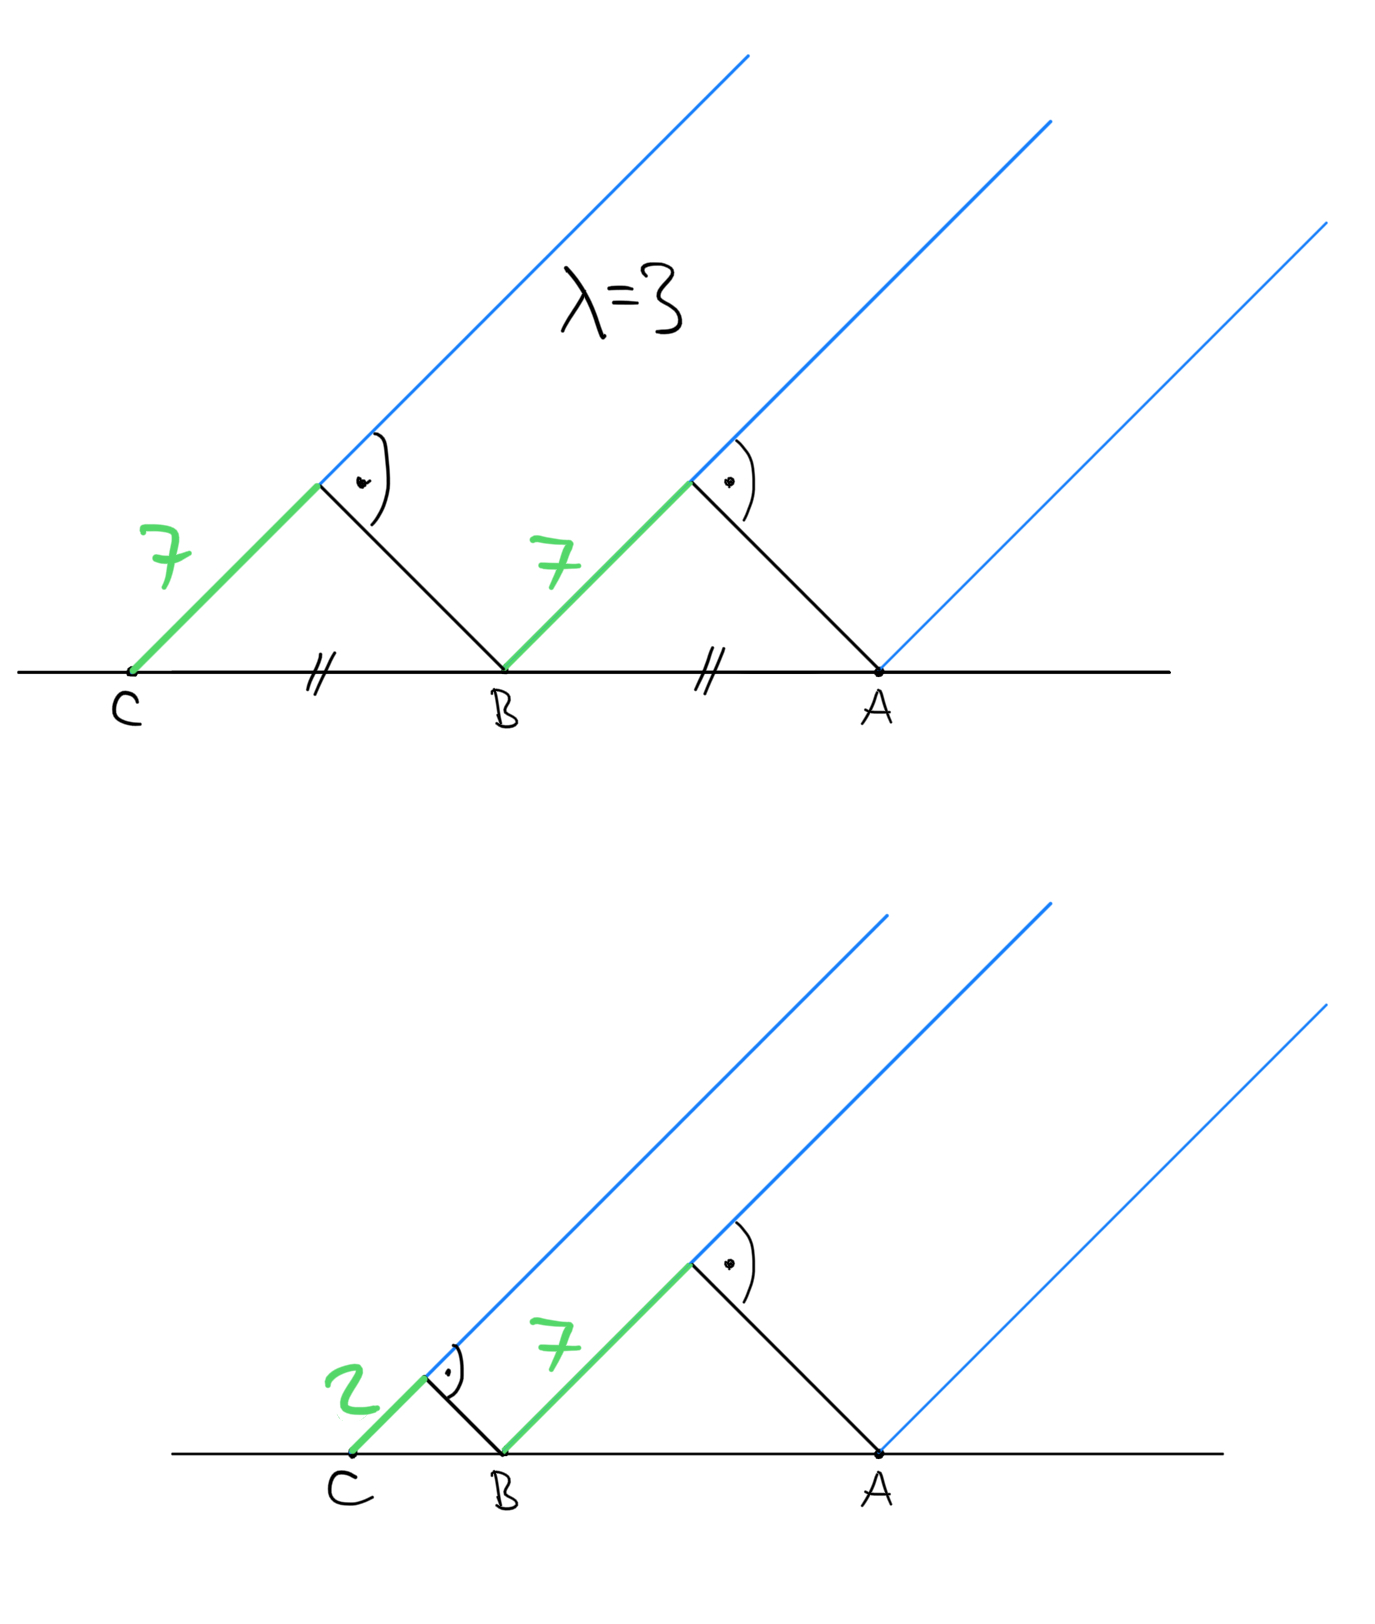
\includegraphics[width=.4\textwidth]{k4.2/baselineunterschied.png}
\caption{Gangdifferenzen von Radiowellen bei Antennenarrays (A,B und C) mit Wellenlänge $\lambda = 3$}
\label{bild-baselineunterschied}
\end{figure}

Zur Kompensation dieses Problems wurde die Radiointerferometrie entwickelt.
Das Verfahren dient zur Überlagerung von Radiowellen, welche von mehreren Antennen aufgezeichnet wurden, um eine höhere Auflösung zu erzielen als es mit einer einzelnen Antenne möglich wäre.
Das hieraus resultierende Signal ist vergleichbar mit dem Signal, welches von einer Antenne mit dem Spiegeldurchmesser entsprechend des Antennenabstandes erzeugt worden wäre.

Ein Interferometer kann nur die Laufzeitdifferenz zwischen Wellen bestimmen, da die einzelnen Wellenberge nicht unterschieden werden können. So können, wie im Beispiel  \cref{bild-baselineunterschied}, bei gleichen Abständen zwischen den Teleskopen A,B und C nicht zwischen den Gangdifferenzen modulo der Wellenlänge, welche im Beispiel $\lambda = 3$ beträgt, unterschieden werden. In diesem Beispiel ist aus den Messwerten nicht ersichtlich, ob es sich tatsächlich um $2\cdot \lambda +1 = 7$ Gangunterschied handelt, sondern jedes $n\in \mathbb{N}$ in $n\cdot\lambda+1$ ist möglich. Die Differenz könnte also immer auch um vielfache von 3 Längeneinheiten verschieden sein. Werden Antennen mit unterschiedlichen Abständen verwendet, sinkt die Anzahl der Kombinationen der Gangunterschiede, für welche sich eine solche Gleichung lösen lässt wie im Beispiel. Hier müssen die Ergebnisse der Gleichung für das untere Bild kongruent zu $3\mathrm{mod}\,2$ sein. Daher werden bei Antennengruppen möglichst viele unterschiedliche Abstände verwendet.

Für die Messung des Radiosignals gilt:
\begin{eqnarray}
d_{uv\lambda} =\int\int I(l,m)e^{-2\pi i \frac{1}{\lambda}(lu-mv)dldm}
\end{eqnarray}
Hier bezeichnet $l$ die Nord-Süd-Achse und $m$ die Ost-West-Achse, $\lambda$ bezeichnet die Beobachtungswellenlänge, und $u$ und $v$ ist der Verbindungsvektor zwischen zwei Antennen. Zusätzlich bezeichnet $n_{uv\lambda}$ ein additives Rauschen. Diese Messgleichung hat große Ähnlichkeit zur Fourier-Transformation (siehe \cref{k4.2.fourier}) und kann als nicht-äquidistante Fourier-Transformation interpretiert werden.

Dieses Verfahren wurde beispielsweise auch beim \emph{Event Horizon Telescope} verwendet. Das \emph{Event Horizon Telescope} besteht aus einer Verschaltung von elf Teleskopen, wobei deren Abstand bis zu $10000\,\text{km}$ beträgt. Mit diesem Teleskop wurde das erste Mal der Schatten eines Schwarzen Lochs beobachtet.

Radiointerferometrie ist also ein essenzieller Bestandteil der Astronomie. Das Verfahren er\-möglicht die Ursprungsbestimmung eines Radiosignals von astrophysikalischen Prozessen bei hoher Auflösung.


\section{Fourier-Transformation}\label{k4.2.fourier}
\sectionauthor{Natalie Teplitska, Ole Fleck, (Constantin Burmeister)}
Bei der Fourier-Transformation handelt es sich um eine mathematische Methode zur Übersetzung eines Signals in ein Frequenzspektrum. Dank ihrer sehr allgemeinen und umfassenden Formulierung findet sie sowohl Anwendung in mathematischen Bereichen, aber auch in der Physik, wie beispielsweise in unserem Kurs bei der Verarbeitung von Radiosignalen.

\begin{figure}
    \centering
    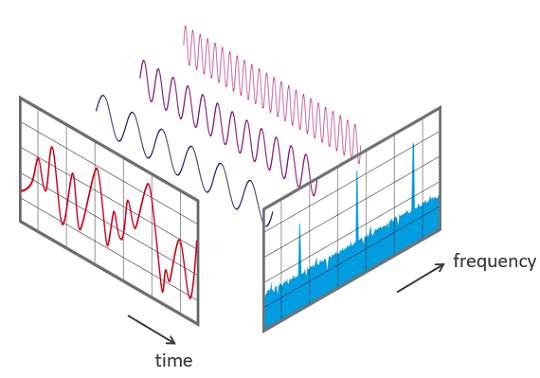
\includegraphics[width=0.6\textwidth]{k4.2/fourier.png}
    \caption{Anschauliche Darstellung der Fourier-Transformation (Quelle: www.nti-audio.com)}
    \label{k4.2.fourier.img}
\end{figure}

Ein anschauliches Beispiel ist die Spektralanalyse von Schallwellen. Die Daten (in der \cref{k4.2.fourier.img} links), die man beispielsweise mit einem Mikrofon aufnimmt, bestehen aus Schallwellen unterschiedlicher Wellenlängen. Mithilfe der Fourier-Transformation wird das Signal auf Schwingungen mit verschiedenen Wellenl\"angen aufgeteilt (in der \cref{k4.2.fourier.img} rechts), wodurch man das Frequenzspektrum erhält.

Je nachdem, welche Art von Rohdaten man erhält und welche Ausgabe erwünscht ist, nimmt die Fourier-Transformation eine leicht andere Form an.

Die kontinuierliche Fourier-Transformation (FT) benötigt als Eingabe eine Funktion, über die mit
\begin{equation}
\mathcal{F}(x)(s)=\int_{-\infty}^{\infty}e^{-ist}x(t)\ dt
\end{equation}
integriert wird. Diese Transformation lässt sich nur auf kontinuierliche Funktionen anwenden und gibt eine kontinuierliche Funktion aus.

Die diskrete Fourier-Transformation (DFT) kommt mit diskreten Werten aus und ist daher am Besten für digitale Signalverarbeitung geeignet, da die Eingabesignale meistens aus einzelnen Datenpunkten und nicht aus kontinuierlichen Funktionen bestehen. Die Formel dazu ist entsprechend kein Integral, sondern eine Summe aller gegebenen Datenpunkte: 
\begin{equation}
\hat a_k = \sum\limits_{j=0}^{N-1}e^{-2\pi i\cdot\frac{jk}{N}}\cdot a_j.
\end{equation}
Die DFT ist mit einer quadratischen Laufzeit allerdings vergleichsweise rechenintensiv. Stattdessen wird in der Signalverarbeitung meist die Fast Fourier Transformation (FFT) verwendet, welche mithilfe des \emph{Divide and Conquer} (Teile-und-Herrsche) Prinzips in der Lage ist, die Rechenzeit drastisch zu reduzieren.

Manche Probleme, welche im Wertebereich, den eigentlichen Signalen, nur durch viele komplizierte Operationen l\"osbar sind, k\"onnen im Bildbereich, dem durch die Fourier-Analyse berechneten Frequenzspektrum, mit wenigen einfachen Operationen gel\"ost werden. Dazu wendet man die Fourier-Analyse auf die Daten an, führt die notwendigen Operationen im Bildbereich aus und transformiert die Lösung zurück in den Wertebereich. Möchte man beispielsweise eine Tonaufnahme von Störsignalen bereinigen, wendet man die FFT an, löscht die unerwünschten Frequenzen im Bildbereich und übersetzt das Ergebnis zurück in Musik oder Sprache. Diese Aufgabe w\"are im Wertebereich erheblich rechenintensiver gewesen, da an einer Tonaufnahme über der Zeit nicht direkt das Störsignal ablesbar ist.

Das \enquote{Rückübersetzen} der Signale erfolgt mit der inversen (kontinuierlichen oder diskreten) Fourier-Transformation (IFT). Diese erzeugt die Funktion oder eine Menge von Datenpunkten, welche aus einem gegebenen Spektrum entsteht. Dazu werden dieselben Operationen wie bei der Berechnung des Spektrums lediglich mit anderen Faktoren angewandt.


\section{Wiener Filter}\label{k4.2.wiener.filter}
\sectionauthor{Constantin Burmeister, Clemens Ljungh, Natalie Teplitska}

Für unseren Kurs benötigen wir eine Möglichkeit, aus Rohdaten auf das zugrundeliegende physikalische Signal zurückzuschließen. Allerdings können Messungen nur mit einer endlichen Sicherheit erfolgen, was bildgebende Verfahren vor Probleme stellt. So lässt sich Rauschen sowie eine gewisse Ungenauigkeit in der Messung nicht vermeiden; zudem sind die Daten unvollständig. Um solche Probleme zu lösen, brauchen wir den Wiener Filter.
Dieses mathematische Verfahren basiert auf dem Bayes'schen Theorem
(\ref{k4.2.bayes})
, welches mathematisch beschreibt, wie Wissen optimal verändert werden muss, nachdem Daten erhoben wurden.

Der Wiener Filter kann nur verwendet werden, wenn die zwei folgenden Annahmen erfüllt sind. Zum Einen setzt man voraus, dass a priori das untersuchte Signal Gauß-verteilt ist: $P(s) = \mathcal{G}(s,S)$. Zum Anderen ist das Rauschen normalverteilt mit $P(n) = \mathcal{G}(n,N)$ und additiv. Aus der Normalverteilung des Rauschens sowie unter Einbezug der Messgleichung ergibt sich auch eine Normalverteilung für die Likelihood. Der Messoperator $R$ muss linear sein. Insgesamt ergibt sich folgende Messgleichung:
\begin{eqnarray}
d = Rs + n
\end{eqnarray}
In der Formel beschreibt $d$ die Daten und $s$ die \emph{Quantity of Interest}, also das ursprüngliche Signal. $R$ ist die Response, das heißt die Abbildung des Signals in den Datenraum. Die Wahrscheinlichkeit, die Daten $d$ für das Signal $s$ zu erhalten, ist eine Gauß-Verteilung.
\begin{eqnarray}
P(d|s) = \mathcal{G}(d-Rs,N)
\end{eqnarray}
Setzen wir $P(s)$ und $P(d|s)$ in Bayes (siehe \cref{k4.2.bayes}) ein, erhalten wir
\begin{eqnarray}
P(s|d) = \mathcal{G}(s-m,D)
\end{eqnarray}
mit
\begin{eqnarray}
D^{-1} = R^{\dagger} N^{-1}R + S^{-1}
\end{eqnarray}
und
\begin{eqnarray}
m = D R^{\dagger} N^{-1}d.
\end{eqnarray}
Der Posterior $P(s|d)$ ist also auch eine Gauß-Verteilung und hat den Erwartungswert $m$. Die Anwendung des Wiener Filters ist für beliebige Datenmengen möglich. Er ist somit eine wichtige Methode der IFT.

\section{Inferenz: Lernen aus Daten}
\sectionauthor{Natalie Teplitska, Clemens Ljungh, Constantin Burmeister}
Mit dem Wiener Filter \cref{k4.2.wiener.filter} besitzen wir ein Werkzeug, unser Wissen über die Welt aufgrund von Daten beständig anzupassen. Allerdings gilt der Wiener Filter nur für den Spezialfall, dass $d=Rs+n, P(s)=\mathcal{G}(s,S), P(n) = \mathcal{G}(n,N)$ gilt.

Unser Ziel ist es, aus Daten das ursprüngliche Signal, welches diese Daten erzeugte, zu rekonstruieren. Dazu müssen wir - bildlich gesprochen - die Formel $d=Rs+n$ invertieren und so das \emph{Signal} $s$ bestimmen. Diese Fragestellung wird als inverses Problem bezeichnet.

Der Posterior ist zwar durch Messgleichung, $P(s)$ und $P(n)$ vollständig definiert, doch seine Berechnung ist insbesondere bei großen Datenmengen, wenn der Posterior nicht analytisch lösbar ist, viel zu rechenintensiv und somit teuer. Zur Bewältigung dieser Herausforderung existieren zwei prominente Lösungsansätze.

Das Verfahren Markov-Chain-Monte-Carlo basiert darauf, dass aus $P(s|d)$ lediglich Stichproben gezogen werden und dadurch eine optimale Lösung gefunden wird. Leider ist auch diese Methode noch zu rechenintensiv, weswegen wir sie nicht nutzen.

Eine weitere Möglichkeit besteht darin, den Posterior lediglich anzunähern. Dieser Ansatz benötigt ein Maß für die Quantifizierung des Approximationsfehlers, welches mit der sogenannten Kullback-Leibler-Divergenz (KL-Divergenz) wie folgt definiert ist:
\begin{eqnarray}\label{k4.2.kldiv}
\text{KL}(P,P_a) = \int P(s|d) \ln \frac{P(s|d)}{P_a(s|d)} ds
\end{eqnarray}
Das Minimieren von $\text{KL}(P, P_a)$ liefert die optimale Approximation an den Posterior.

Die KL-Divergenz hat einige nennenswerte Eigenschaften. Dazu gehört unter anderem die Lokalität, die dazu führt, dass nur Stellen in die Fehlerberechnung einfließen, über welche die erste Verteilung $P$ eine Aussage trifft. Außerdem folgt die KL-Divergenz dem Prinzip der Gescheitheit, welches besagt: \enquote{Wann immer möglich, wähle die zweite Verteilung $P_a$ so, dass diese mit der ersten übereinstimmt}. Zuletzt ist zu erwähnen, dass die KL-Divergenz invariant unter Koordinatentransformationen ist und sich daher nicht verändert, wenn die Koordinatenachsen transformiert werden.

Die KL-Divergenz wendet man bei der variativen Inferenz an. Dabei minimiert man jedoch nicht $\text{KL}(P, P_a)$, sondern $\text{KL}(P_a, P)$, da diese Optimierung weniger rechenintensiv ist. Die Optimierungen im Folgenden minimieren die variative $\text{KL}(P_a, P)$.


\section{Hierarchisches Modell für korrelierte Felder}\label{k4.2.hiera}
\sectionauthor{Natalie Teplitska, Clemens Ljungh, Constantin Burmeister}
Im Folgenden wird der Prior $P(s)$ für die Radioastronomie und Tomographie diskutiert. In unserem Modell müssen wir glatte Signale $s$ darstellen können. Eine besonders einfache Art,, diese zu formulieren ist über einen hierarchischen Aufbau. Zu diesem Zweck wird im Folgenden die Python Bibliothek \emph{NIFTy8} benutzt.

Ziel eines bildgebenden Verfahrens ist die Bestimmung von $s$. Dies kann bei der Radioastronomie die Helligkeit des Himmels oder bei der CT die Dichte des untersuchten Objektes sein. Da weder Helligkeit noch Dichte negativ sein kann, setzen wir $s \geq 0$ voraus. Damit lässt sich eine Normalverteilung für $P(s)$ bereits ausschließen, da eine solche über ganz $\mathbb{R}$ definiert wäre. Außerdem wird angenommen, dass die einzelnen Bildpunkte miteinander korreliert sind, also voneinander abhängen. Ist zum Beispiel ein Pixel dunkel, so ist es unwahrscheinlich, dass sich in direkter Nähe dazu helle Pixel befinden. In unserem Fall gilt, dass die Abhängigkeit zunimmt, je kleiner dar Abstand zwischen zwei Pixeln ist. Daraus ergibt sich eine schwierig darzustellende Kovarianzmatrix, die die Korrelation der Pixel zueinander codiert.

Wir reduzieren die Komplexität von $s$, indem wir eine weitere hierarchische Stufe ergänzen. Als Zufallsvariable wird statt $s$ nun $\xi$ verwendet, welches mit $P(\xi) = \mathbb{G}(\xi, \mathds{1})$ standard-nor\-mal\-ver\-teilt ist.

Unsere Aufgabe bestand nun darin, eine Funktion $f$ so zu definieren und zu implementieren, sodass $P(f(\xi)) d \xi = P(s) ds$. Die Schwierigkeit besteht in der Codierung der Kovarianzmatrix in $f$.

Die \emph{Cholesky-Zerlegung} stellt eine Möglichkeit dar, ein solches $f$ zu erzeugen, wobei nur eine Dreiecksmatrix mit halb so vielen Einträgen gespeichert werden muss. Anschaulich gesprochen ziehen wir aus $s$ die Wurzel, sodass $S=A A^{\dagger}$. Auf diese Weise lässt sich eine Funktion definieren, die aus zufälligen Zahlen $\xi$ den Prior über $s$ berechnet: $s = f(\xi) = A \cdot \xi$. Allerdings ist der Speicherverbrauch der Dreiecksmatrix für $\mathcal{O}(100 000)$ Datenpunkte immer noch enorm.

Einen alternativen Ansatz stellt das \emph{Wiener-Chintchin-Theorem} dar. Hier wird die Annahme getroffen, dass die Kovarianz zwischen den Pixeln nur von deren Entfernung, nicht jedoch von deren Position abhängt. Dabei gilt
\begin{eqnarray}
S= \mathcal{F}^{\dagger} diag(p(|k|)) \mathcal{F} \ .
\end{eqnarray}
Wir haben damit erfolgreich die Kovarianzmatrix in eine diagonale Form gebracht: das Powerspektrum $diag(p(|k|))$. Mit der Hartley-Transformation \footnote{Variante der Fourier-Transformation, welche Real- und Imaginärteil im reellen Raum verrechnet} übersetzen wir vom Raum des Powerspektrums zum Raum der Kovarianzmatrix.

Bisher haben wir mit einer vorgegebenen Kovarianz $S$ gearbeitet. Um aus Daten lernen zu können, wollen wir uns allerdings nicht auf eine bestimmte Kovarianzmatrix festlegen. Die Berechnung des Posteriors gestaltet sich wesentlich einfacher, wenn das Powerspektrum über eine Menge von Parametern definiert wird. Diese können jeweils mit Bayes (siehe \cref{k4.2.bayes}) immer weiter angepasst werden. Für unseren Fall arbeiteten wir mit drei Parametern (siehe \cref{k4.2.power-function.img}).
\begin{figure}
    \centering
    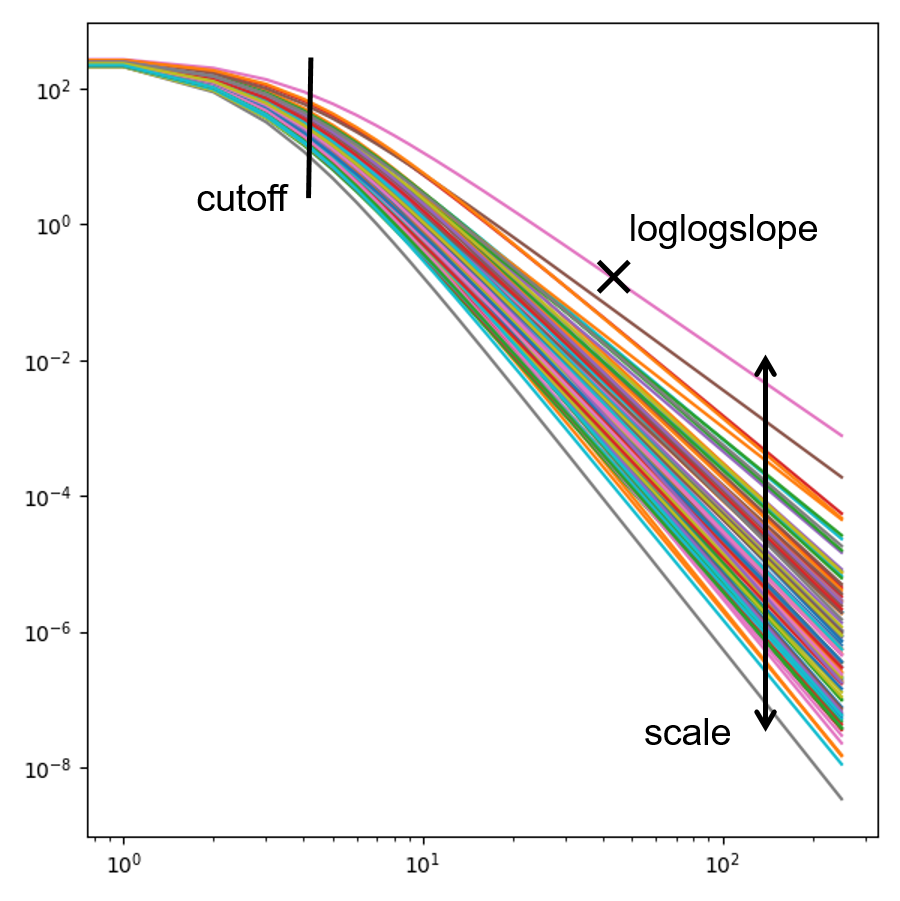
\includegraphics[width=0.4\textwidth]{k4.2/power_function_bearbeitet.png}
    \caption{100 beispielhafte power functions und ihre Parameter}
    \label{k4.2.power-function.img}
\end{figure}
\begin{itemize}
    \item Der Parameter \emph{scale} steht für die Standardabweichung des Powerspektrums und beschreibt somit, wie stark es variieren kann.
    \item Wir gehen von einer Funktion aus, die rechts von einem bestimmten Punkt eine Form annimmt, welche einem power-law folgt. Diesen Punkt bezeichnet man als \emph{cutoff}.
    \item Schließlich bezeichnet \emph{loglogslope} die Steigung der Funktion in dem Intervall nach dem cutoff.
\end{itemize}
Alle drei Parameter werden über je zwei Zahlenwerte definiert: den Mittelwert der Erwartungen und seine vermutete Varianz. Im Grunde genommen arbeiten wir also mit sechs Zahlenwerten, die unter Einbezug von Daten immer weiter angepasst werden können.

Damit haben wir es geschafft, einen Prior für $s$ mittels a priori sehr einfach verteilten Zufallszahlen zu generieren, der ein Lernen aus Daten mit kleinstmöglichem Rechen- und Speicheraufwand ermöglicht.



\section{Radiointerferometrie-Response und Event-Horizon-Telescope-Daten}
\sectionauthor{Lara Müller, Alexander Gitnik, Jonas Fiedler, Patricia Hackl}

Zur Rekonstruktion eines Bildes des Schwarzen Lochs M87* muss basierend auf den Daten des Event-Horizon-Telescopes zunächst eine Response-Funktion implementiert werden, um die Informationen vom Signal- in den Datenraum zu transferieren $s \mapsto d$. Mit der entsprechenden Implementierung wird sich der nachfolgende Abschnitt befassen.

Es werden Daten in Form von acht csv-Dateien verwendet, die im April 2017 aufgenommen wurden. Diese stammen von mehreren Messreihen und wurden zur weiteren Verarbeitung in Form von csv-Dateien gespeichert.
Um mit den Messwerten in Python arbeiten zu können, werden die csv-Dateien in NumPy-Arrays konvertiert. Durch das NumPy-Array werden die Daten aus den csv-Dateien auf einem zweidimensionalen Gitter abgebildet.

Zunächst müssen die Frequenzen der Radiowellen ausgelesen werden. Diese elektromagnetischen Wellen werden in unmittelbarer Nähe des Schwarzen Lochs ausgesandt. Es wurden die beiden Frequenzen $f_1 = 227.0707$ GHz und $f_2 = 229.0707$ GHz betrachtet. Darüber hinaus werden auch die Verbindungsvektoren zwischen den Antennen $uvw$ ausgelesen.

Um aus den Messwerten ein Bild erstellen zu können, wird die Anzahl der Pixel sowohl in x-, als auch in y-Richtung auf zunächst $100$ festgelegt, wobei dieser Wert variabel ist. Die Größe der Pixel ergibt sich für $\delta \theta$:
\begin{equation}
\delta \theta = 1.22 \cdot \displaystyle\frac{\lambda}{D} = 1.22 \cdot \displaystyle\frac{c}{f \cdot D}
\end{equation}
Da es sich bei dem Event Horizon Telescope um einen Zusammenschluss von Antennen auf der ganzen Welt handelt, ergibt sich ein Durchmesser von $D_{EHT} \approx D_{Erde} \approx 10.000\text{km}$. Desweiteren beschreibt $\lambda$ die Wellenlänge der Radiowellen und $c$ deren Ausbreitungsgeschwindigkeit, die der Lichtgeschwindigkeit entspricht. In die Formel eingesetzt erhält man:

\begin{equation}
  \delta \theta = 1.22 \cdot \displaystyle\frac{3 \cdot 10^{8} \displaystyle\frac{\text{m}}{\text{s}}} {229.0707 \text{GHz} \cdot 10000 \text{km}} = (1.598 \cdot 10^{-10}) \mu \text{as} 
\end{equation}

Damit ein erstes Bild des Schwarzen Lochs generiert werden kann, ist es notwendig, die Daten $d$ mittels folgender Formel zu beschreiben. Die Werte für $I_{Amplitude}$ und $I_{Phase}$ sind in den csv-Dateien gegeben:
\begin{equation}
d = I_{Amplitude} \cdot e^{i \cdot I_{Phase}}
\end{equation}

Aufgrund unvollständiger Informationen, die durch die Distanz der Antennen des Event-Horizon-Telescopes entstehen, muss zur Bilderstellung Bayes'sche Statistik angewandt werden. Im Gegensatz zu NumPy stellt NIFTy entsprechende Funktionen bereit, die dies ermöglichen. Um vom Signalraum $I$ (Signal des betrachteten Objekts) in den Datenraum $d$ (empfangene Daten) zu gelangen, nutzt man in NIFTy die Funktion \verb|dirty2vis| aus der Python-Bibliothek \verb|ducc0|. Diese ist vergleichbar mit der Response $R$ beim Wiener Filter. $R^{\dagger}$ entspricht der adjungierten Abbildung \verb|vis2dirty|, die es ermöglicht, aus dem bekannten Datenraum auf den Signalraum zu schließen.

Um diese Funktionen in NIFTy wiederholt anwenden zu können, werden sie in eine Klasse verpackt. Es handelt sich dabei um eine Klasse, die von \verb|ift.LinearOperator| - einem NIFTy-Operator - erbt. Dazu müssen unter Anderem \verb|domain| und \verb|target| initialisiert werden. Der Signalraum wird über \verb|domain| beschrieben, der Datenraum über \verb|target|. In der Klasse werden die Funktionen \verb|dirty2vis| und \verb|vis2dirty| durch die Methoden \verb|TIMES| und \verb|ADJOINT_TIMES| ersetzt.

Die hieraus resultierende Datensätze können nun als Grundlage für eine Approximation an das wahre Signal dienen.



\section{Radiointerferometrie}
\sectionauthor{Benjamin Knöbel del Olmo, Ole Fleck, Aaron Gschwendt, Mara Germann}
\subsection{Kalibrierung der Radiointerferometriedaten}
Das Ziel dieses Projektteils ist es, Kalibrierungsfehler aus den Interferometriedaten herauszuprojizieren. Im Gegensatz zu Beobachtungen durch einzelne Antennenarrays wurde das Schwarze Loch M87* durch das Event-Horizon-Telescope (EHT) vermessen. Das EHT besteht aus Antennenstationen in verschiedensten Ländern (Chile, Spanien, Hawaii etc.). Der Abstand zwischen den Stationen ermöglicht es, sehr kleine Winkel aufzulösen (\cref{k4.2.radioformel}).
Bei der Messung treten vor allem zwei systematische Effekte vor: Dynamiken in der Atmosphäre führen zu Phasenverschiebungen und Temperaturschwankungen im Empfänger verursachen eine zeitabhängige Skalierung der Messdaten. Diese Störungen lassen sich durch die Formel
\begin{equation}
d_{abt\lambda}\rightarrow g_{at\lambda} \bar{g}_{bt\lambda}d_{abt\lambda}, \hspace{1cm} g_{at \lambda} \in \mathbb{C} \quad \forall a,t,\lambda
\end{equation}
darstellen, wobei $a$ und $b$ für ein betrachtetes Antennenpaar (also Antenne $a$ und Antenne $b$) stehen und $g_{at\lambda}$,  $g_{bt\lambda}$ zwei für die jeweilige Antennenstörung beschreibende komplexe Zahlen sind: Der Abstandsbetrag spiegelt die Signalstärkenreduktion wider, während die komplexe Phase die Phasenverschiebung repräsentiert.
Um diese Effekte herauszukürzen, bestimmen wir die \emph{Closure Phases} und \emph{Closure Amplitudes}, eine bereinigte Form der gegebenen Daten. \emph{Closure Phases} behandeln die Phasenverschiebung der empfangenen Welle und \emph{Closure Amplitudes} die Änderung der Signalstärke. Für die Konstruktion der \emph{Closure Quantities} muss eine Funktion $f_{\lambda}$
\begin{equation}
d^0_{t\lambda}=f_{\lambda}(d_{ab\lambda},\quad \forall a,b)
\end{equation}
gefunden werden, die invariant ist unter
\begin{align}
d_{abt\lambda} &\rightarrow e^{i \phi_{at}} e^{-i\phi_{bt}} d_{abt\lambda}d(0)\\
d_{abt\lambda}&\rightarrow|g_{at\lambda}||g_{bt\lambda}|d_{abt\lambda}|
\end{align}
In der ersten Funktion werden die Verschiebungen in der Phase rausgekürzt, in der zweiten die Amplitudenverschiebung.
Für die \emph{Closure Phases} lautet eine geeignete Funktion
\begin{equation}f(d_{a,b},d_{b,c},d_{a,c})=d_{a,b}+d_{b,c}-d_{a,c}\end{equation}
Man kann zeigen, dass durch Einsetzen in die Funktion die Verschiebung der Daten herausgerechnet wird. 
Sei $\psi_n = e^{i \phi_{nt}}$ Dann gilt:
\begin{align}
f(\psi_a\bar{\psi_b} d_{a,b},\psi_b\bar{\psi_c}d_{b,c},\psi_a \bar{\psi_c} d_{a,c})&=\psi_1\bar{\psi_b}d_{a,b}+\psi_b\bar{\psi_c}d_{b,c}-\psi_a \bar{\psi_c} d_{a,c}\\
&=e^{i \phi_{a,t}-i\phi_{b,t}}d_{a,b}+e^{i \phi_{b,t}-i\phi_{c,t}}d_{b,c}-e^{i \phi_{a,t}-i\phi_{c,t}}d_{a,c}\\
&=d_{a,b}+d_{b,c}-d_{a,c}\\
&=f(d_{a,b},d_{b,c},d_{a,c}).
\end{align}
Für die \emph{Closure Amplitudes} lauten zwei mögliche Funktion:
\begin{align}
f(d_{a, b},d_{a, c},d_{a, d},d_{b, c},d_{b, d},d_{c, d})\overset{!}{=}\frac{d_{a,b}\cdot d_{c,d}}{d_{a,c} \cdot d_{b,d}}
\hspace{3mm}\text \quad {bzw.} \quad \hspace{3mm} \frac{d_{a,d}\cdot d_{b,c}}{d_{a,c} \cdot d_{b,d}}
\end{align}
Folgend werden die \emph{Closure Phases} für die verschiedenen Dreiergruppen bzw. die \emph{Closure Amplitudes} für die Vierergruppen aus Antennenpaaren berechnet. Da jedoch nicht alle Möglichkeiten unabhängig voneinander sind, müssen Redundanzen herausgerechnet werden.
Dafür wird eine Matrix erstellt, in der die Spalten alle möglichen Antennenpaare darstellen und die Zeilen alle linear unabhängige Möglichkeiten, die Antennenpaare zu verknüpfen, darstellt. Bei den  \emph{Closure Phases} stehen die Zahlen in der Matrix für das Vorzeichen, bei den \emph{Closure Amplitudes} für das Vorzeichen des Exponents. Folglich bedeuten Nullen, dass die Antennenpaare nicht verwendet werden.  Bei $n$ Antennen gibt es $\binom{n-1}{2}= \frac{1}{2}(n-1)(n-2)$ linear unabhängige Zeilen in der Matrix. 
Daher hat die $n=4$ \emph{Closure-Phase}-Matrix $\binom{4-1}{2}=3$ Zeilen:
\begin{equation}
\bordermatrix{
~ &(0,1)&(0,2)&(0,3)&(1,2)&(1,3)&(2,3)\cr
~&1&-1&0&1&0&0 \cr
~&1&0&-1&0&1&0 \cr
~&0&1&-1&0&0&1 \cr}
\end{equation}

Die \emph{Closure-Amplitude}-Matrix von $n$ Antennen hat $\frac{1}{2}n(n-3)$ linear unabhängige Reihen. Die $n=4$ \emph{Closure-Amplitude}-Matrix sieht folgendermaßen aus:
\begin{equation}
\bordermatrix{
~ &(0,1)&(0,2)&(0,3)&(1,2)&(1,3)&(2,3)\cr
~&1&-1&0&0&-1&1 \cr
~&0&-1&1&1&-1&0 \cr
}
\end{equation}
Um die \emph{Closure Phase} Matrizen zu generieren, verwenden wir folgende Funktion. 
\begin{verbatim}
def genPhaseMatrix(n):
    O=math.comb(n,2)
    mat=np.empty(O,dtype=int)
    pos=[(x,y) for x in range(n) for y in range(x+1,n)]
    maxRank=math.comb(n-1,2)
    for i in range(0,n):
        for j in range(i+1,n):
            for k in range(j+1,n):
                row=np.zeros(O,dtype=int)
                row[pos.index((i,j)),]=1
                row[pos.index((i,k))]=-1
                row[pos.index((j,k))]=1
                newMat=np.vstack([mat,row])
                rnk= np.linalg.matrix_rank(newMat)
                if rnk>np.linalg.matrix_rank(mat):
                    mat=newMat
                    if rnk==maxRank:
                        return mat[1:,:]
\end{verbatim}
Die Funktion nimmt als Parameter die Anzahl an Antennen. Zunächst erstellt sie ein leeres Numpy-Array mit einer Zeile für jedes mögliches Antennenpaar. In dem Array wird die Matrix zeilenweise erzeugt. Dann werden alle mögliche Kombinationen von drei Antennen durchlaufen. Ist die Kombination linear unabhängig zu der bereits bestehende Matrix, wird sie der Matrix zugefügt. Dies wird so oft wiederholt, bis entweder alle Möglichkeiten durchgegangen oder die maximale Zeilenanzahl der Matrix erreicht wird. \emph{Amplitude-Phase}-Matrizen werden analog generiert.

Nachdem die \emph{Closure Quantities} erstellt wurden, werden die Daten der Antennen für jedes Zeitintervall in Phase und Amplitude getrennt und mit den \emph{Closure Quantities} Matrizen multipliziert. Da nicht zu jedem Zeitpunkt gleich viele Antennen aktiv sind, (z.B. weil sie im Schatten der Erde liegen) brauchen wir alle \emph{Closure}-Matrizen bis $n=7$ gilt.

Um schließlich ein Bild zu erzeugen, benötigen wir den Posterior aus dem Theorem von Bayes. Um diesen zu berechnen, setzen wir ein: 


\begin{equation}
P(\xi|d)= \frac {P(d|\xi)\cdot P(\xi)}{ P(d) }
\end{equation}

\begin{equation}
P(d|\xi)=  {P(d_{ph}|\xi)\cdot P(d_{amp}|\xi)}    
\end{equation}

Die Likelihood (\cref{k4.2.likelihood}) besteht aus zwei Teilen: $P(d_{ph}|\xi)$, der Wahrscheinlichkeit der \emph{Closure Phases} gegeben die Parameter $\xi$ und $P(d_{am}| \xi)$, der Wahrscheinlichkeit der \emph{Closure Amplitudes} gegeben $\xi$ : 

Der negative Logarithmus des Posteriors
\begin{align} \label{k4.2.Posterior}
 -\log {P(\xi|d)} &= 
 \mathcal{H} (\xi|d) = \mathcal{H} (d_{ph}|\xi)+\mathcal{H} (d_{amp}|\xi)+\mathcal{H} (\xi) \\
&= \frac {1}{2}\cdot \Bigg[d_{ph} - f_{ph}(R(sky(\xi))) \Bigg]^\dagger N^{-1}_{ph} \Bigg[d_{ph} - f_{ph}(R(sky(\xi))) \Bigg] 
\\  & + \frac {1}{2}\cdot \Bigg[d_{amp} - f_{amp}(R(sky(\xi))) \Bigg]^\dagger N_{amp}^{-1}\Bigg[d_{ph} - f_{ph}(R(sky(\xi))) \Bigg] \nonumber
\\ & +  \frac {1}{2} \cdot \xi^\dagger \xi \nonumber  
\end{align} 
 erlaubt uns, Metric Gaussian Variational Inference, kurz MGVI \parencite{k4.2.mgvi} anzuwenden. Dabei wird der Parameter $\xi$ so optimiert, dass man mit einer durch $\xi$ definierten Normalverteilung eine möglichst kleine Differenz zum wahren Posterior erreicht \cref{k4.2.hiera}
Dadurch erhält man folgendes Bild:

\begin{figure}
    \centering
    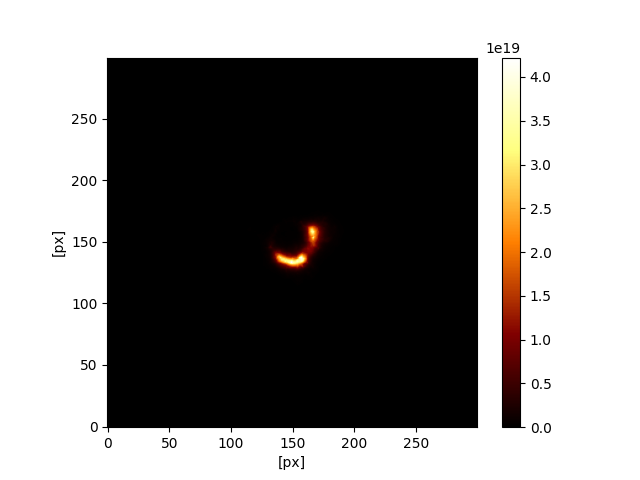
\includegraphics[width = 0.9\textwidth]{k4.2/black-hole-lin.png}
    \caption{Bild des Schwarzen Lochs M87*}
    \label{k4.2.black-hole-lin}
\end{figure}



\section{Tomographie}\label{k4.2.comptomo.ct}
\sectionauthor{Aaron Gschwendt, Finja Hoffmann}

Die Tomographie ist ein bildgebendes Verfahren, in dem ein Objekt schichtweise untersucht wird. Um diese Schichten zu vermessen, beobachtet man Strahlen, die das Objekt schneiden und auf einer Ebene liegen. Die Menge an Licht, die auf der Strecke absorbiet wurde, entspricht dem Linienintegral:

$$d=\int_{\Gamma}{}s(p)dp(\gamma)$$

$s$ ist eine unbekannte Funktion, die jedem Punkt im Raum eine optische Dichte zuordnet. $d$ ist das Linienintegral von $s(p)$ entlang dem Pfad $\gamma$. $d$ entspricht der Menge an Licht, die zwischen dem Sender und dem Empfänger absorbiert wird und wird experimentell bestimmt.

Gesucht ist die Funktion $s$, diese lässt sich jedoch nicht analytisch bestimmen. Kennt man aber $d$ von genug Linien in $s$, kann man mithilfe des Satzes von Bayes mit hoher Auflösung und Sicherheit $s$ bestimmen.

\subsection{Staubtomographie}

In der Astronomie wird die Tomographie z.B. verwendet, um die Form von kosmischen Wolken zu ermitteln. Dafür werden Sterne, deren absolute Helligkeit und Distanz bekannt ist beobachtet. Man vergleicht ihre scheinbare Helligkeit mit der zu erwartende Helligkeit und ermittelt so $d$ für alle Strecken zwischen der Erde und den beobachteten Sternen. $d$ entspricht in dem Fall die Menge an Staub zwischen dem Stern und der Erde. Aus vielen (Distanz, Helligkeit)-Paaren kann man $s$ lernen und Aussagen über die dichte-Verteilung und Form der Wolke treffen.

\subsection{Computertomographie}\label{k4.2.comptomo}

Häufig verwendet wird die Tomographie auch in der Medizin, bekannt als Computertomographie(CT).

Bei herkömmlichen Röntgenuntersuchungen wird Röntgenstrahlung durch das abzubildende Objekt auf einen Röntgenfilm oder einer Sensorplatte geleitet. Das 3d-Objekt wird dabei auf eine 2d-Fläche projiziert. Der Nachteil dieser Methode ist, dass sich Teile vom Objekt überlagern können und nicht erkannt werden kann, ob es sich um ein Objekt mit hoher Absorption oder mehrer Objekte mit geringer Absorption handelt.

Beim CT drehen sich im $180^\circ$ Winkel eine Röntgenröhre und Detektor um den Patienten und nehmen dabei in kleinen Abständen Messpunkte auf. Dies wird für mehrere Schichten entlang des zu untersuchenden Körperteils ausgeführt. Der Röntgenstrahl und Detektor ist so breit, dass bei jedem Messpunkt die ganze Breite des Körperteils in einem Streifen ergriffen wird.

\begin{figure}
 \centering
 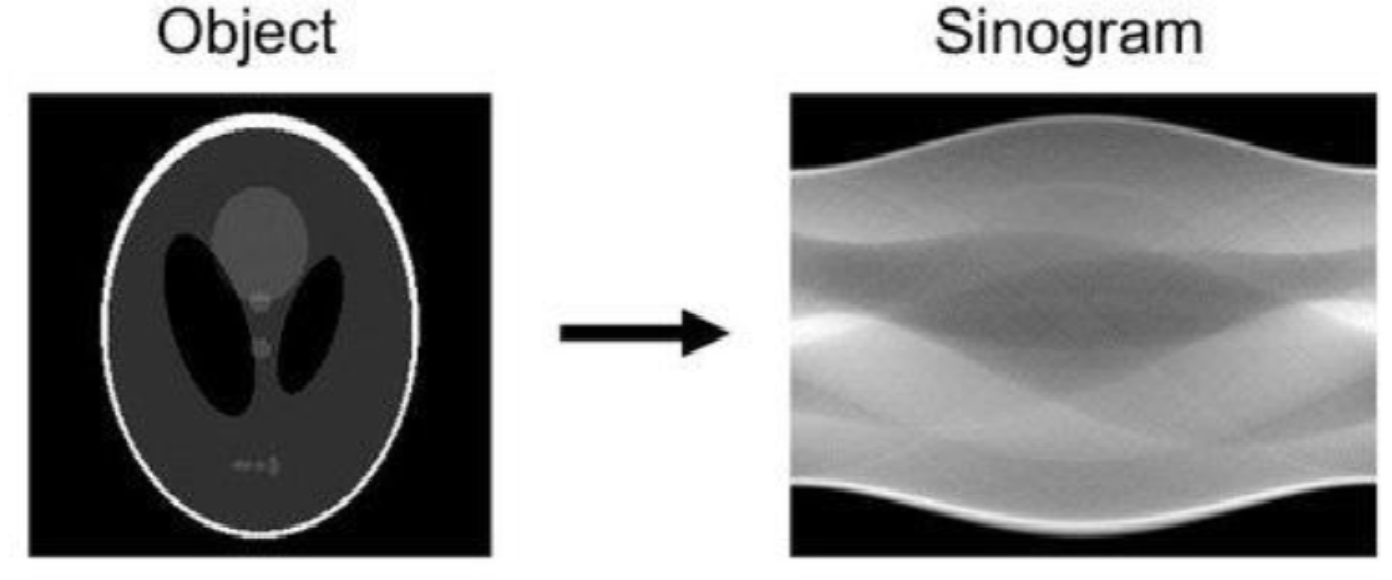
\includegraphics[width=0.4\textwidth]{k4.2/backprojektion.png}
 \caption{Abbildung eines Objektes als Sinogram}
 \label{k4.2.tomo.ct.bp}
\end{figure}

Daraus entsteht für jede Schicht ein Sinogram \cref{k4.2.tomo.ct.bp} bei der eine Achse (hier Y-Achse) das Absorptionsprofil und die andere (hier X-Achse) dem Winkel entspricht. Jede Stelle im Objekt bildet eine Sinuskurve; ihr Abstand vom Mittelpunkt entspricht der Amplitude und ihr Winkel im vergleich zum Startpunkt der Phasenverschiebung der Sinuskurve. Mit dem bayeschen Verfahren  kann man ein Bild von der Schicht mit hoher Genauigkeit rekonstruieren. Führt man dies für jede durch, Schicht erhält man ein 3d-Rendering des Objekts.


\subsection{CT in 3D}\label{k4.2.ct.3d}
\sectionauthor{Finja Hoffmann, Chuyang Wang}

Im Rahmen der Projektarbeit soll aus den gemessenen Daten $d$ die Funktion des Signals $s(p)$ (\emph{quantity of interest}) in Abhängigkeit von einem 3D-Punkt $p \in \mathbb{R}^3$ rekonstruiert werden, welche die Dichte eines Objekts in einem diskreten 3-dimensionalen Raum beschreibt. Generell lässt sich der Datenvektor $d \in \mathbb{R}^N$ wie folgt berechnen:

\begin{equation}
  \label{k4.2.ct.3d.datamodel}
  \begin{aligned}
    d = Rs + n,
  \end{aligned}
\end{equation}

wobei $R \in \mathbb{R}^{N \times M}$ die \emph{Response}, $s \in \mathbb{R}^M$ das Signal und $n \in \mathbb{R}^N$ das Rauschen beschreiben. 
% TODO: ref to Wiener Filter

\subsection{Line-Of-Sight Response}\label{k4.2.ct.resp}

Angenommen, die Start- und Endpunkte der Messungen seien bereits gegeben und bilden jeweils die Strecken. Aus diesen Daten kann man die Matrix $R$ konstruieren. Anders gesagt repräsentiert $R$ die Start- und Endpunkten. Da das Signal (die Dichtenverteilung) in Form von diskreten 3D-Pixel angegeben sind, ist $R$ eine Matrix der Gewichte der gegebenen Komponenten des Signals. Als Gewichtung eines Datenwürfels gilt der euklidischen Abstand zwischen den beiden Schnittpunkten der Strecke mit den Seiten des Würfels. \textcite{k4.2.siddon} hat dafür einen effizienten Algorithmus geliefert, dessen Ansatz hier umgesetzt wird.


\subsection{Algorithmus von Siddon}\label{k4.2.ct.siddon}

Siddons Ansatz nach könnte man die Schnittpunkte einer Sichtlinie mit den x-, y- und z-Achsenebenen jeweils einzeln bestimmen und in sortierte Listen $A$, $B$ und $C$ speichern. Sei jeweils

\begin{equation}
  P_{start} = \begin{pmatrix}x_{start} \\ y_{start} \\ z_{start}\end{pmatrix}
\end{equation}

\begin{equation}
  P_{end} = \begin{pmatrix}x_{end} \\ y_{end} \\ z_{end}\end{pmatrix}
\end{equation}

Betrachtet man zunächst die x-Achsenebene. Ohne Beschränkung der Allgemeinheit sei $x_{start} < x_{end}$. Man rundet die x-Koordinate des Startpunktes in die Richtung der Strecke auf und berechnet die Differenz $x^{\ast}$. Um die y- und z-Koordinaten dieses ersten Schnittpunkts herauszufinden, muss man noch die Steigungen gegenüber dieser beiden Achsen $m_{yx} = \frac{y_{end} - y_{start}}{x_{start} - x_{end}}$ und $m_{zx} = \frac{z_{end} - z_{start}}{x_{start} - x_{end}}$ berechnen. Somit erhält man den ersten Schnittpunkt

\begin{equation}
  S_{x,0} = \begin{pmatrix}
    x_{start} + x^{\ast} \\
    y_{start} + x^{\ast} \cdot m_{yx} \\
    z_{start} + x^{\ast} \cdot m_{zx} \\
  \end{pmatrix}.
\end{equation}

Die weiteren Schnittpunkte $S_{x,i}$ kann man rekursiv konstruieren, indem man jeweils eine Einheit in die x-Richtung geht und die Änderungsrate gegenüber der y- und z-Achsen jeweils aufaddiert

\begin{equation}
  S_{x,i} = S_{x,i-1} + \begin{pmatrix}
    1 \\
    1 \cdot m_{yx} \\
    1 \cdot m_{zx} \\
  \end{pmatrix}.
\end{equation}

 Die Liste $A$ besteht aus allen Schnittpunkten $[S_{x,0}, S_{x,1}, ..., S_{x,n}]$ mit x-Ebenen. Die Listen $B$ und $C$ berechnet man analog.

Anschließend muss man die drei Listen in eine einzelne sortierte Liste $\mathbf{S}$ zusammenführen. Diese geschieht, indem man alle Schnittpunkte aus $A$, $B$ und $C$ nach den x-Koordinaten aufsteigend sortiert. Sollte $x_{start} = x_{end}$ sein, dann nutzt man die y- oder z-Achse als den Sortierschlüssel.

Hat man alle sortierten Schnittpunkte, so kann man auch die Gewichtungen, i.e. die Abstände zwischen den jeweiligen Punkten, einfach berechnen. Jede dieser Gewichtungen wird einem 3D-Pixel zugeordnet, durch den diese Teilstrecke durchdringt. Für diese Sichtlinie kann dann ein Zeilenvektor $r_i$ erstellt werden, welcher diese Zuordnung von Gewichtungen speichert. Man beobachte, dass jede Sichtlinie nur wenige Pixeln im 3D-Raum durchgeht. Die meisten Gewichte für die diskretisierte Dichtenverteilung entlang einer Sichtlinie sind null.


\subsection{Walnuss CT-Messdaten}\label{k4.2.ct.walnuss}
\sectionauthor{Leo Bergmann, Cedric Balzer}
\begin{figure}
	\centering
	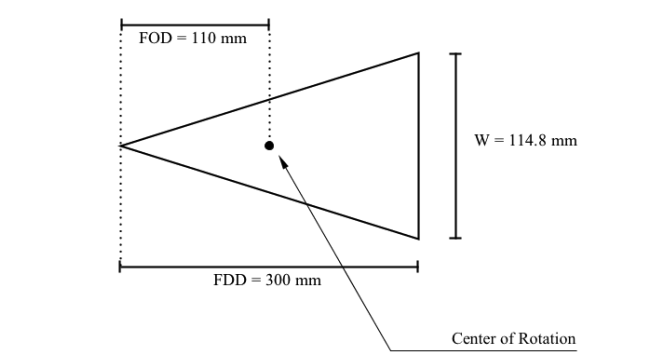
\includegraphics[width=0.7\textwidth]{k4.2/geometry.png}
	\caption{Aufbau des Versuchs mit dessen Geometrie aus \textcite{k4.2.hamalainen2015tomographic}.
	FOD steht für \enquote{Focus-to-object} distance, FDD für \enquote{Focus-to-detector} distance und W für die Breite des Detektors.
	}
	\label{k4.2.fig.geo}
\end{figure}

Das Ziel des Projekts ist es ein Bild einer Walnuss, anhand von CT-Scandaten (siehe \cref{k4.2.comptomo}), zu rekonstruieren. Die Herausforderung besteht darin die Unsicherheit in der DIchteverteilung des zu vermessenden Objekts zu quantifiziern. Aus ein Bayes'schen Perspektive (siehe \cref{k4.2.bayes}) quantifiziert der Posterior die Unsicherheit. Die präzise Beschreibung ist bei medizinischer Bildgebung wichtig.
Die Daten, auf welchen unser Projekt beruht, enthalten Sinogramm und Schichtaufnahme einer Walnuss, welche in \verb|.mat|-Dateien gespeichert sind \parencite{k4.2.hamalainen2015tomographic}.
In dem Versuch wurde eine Walnuss zwischen eine punktförmige Strahlungsquelle und einen flachen Schirm positioniert (\cref{k4.2.fig.geo}). Nach jeder Messung wurde die Nuss um 3° gegen den Uhrzeigersinn gedreht.
Insgesamt wurden 120 Messungen durchgeführt. Diese Daten wurden auf 328 Pixel herunterskaliert und in einer Matrix \verb|m| gespeichert.
Damit das Sinogramm in ein Bild der Dichteverteilung zurückprojeziert werden kann sind alle Start- und Endpunkte der Sichtline notwendig. Diese errechnen sich aus der Position der Quelle und der Position der einzelnen Pixel des Screens.\\


\begin{figure}
	\centering
	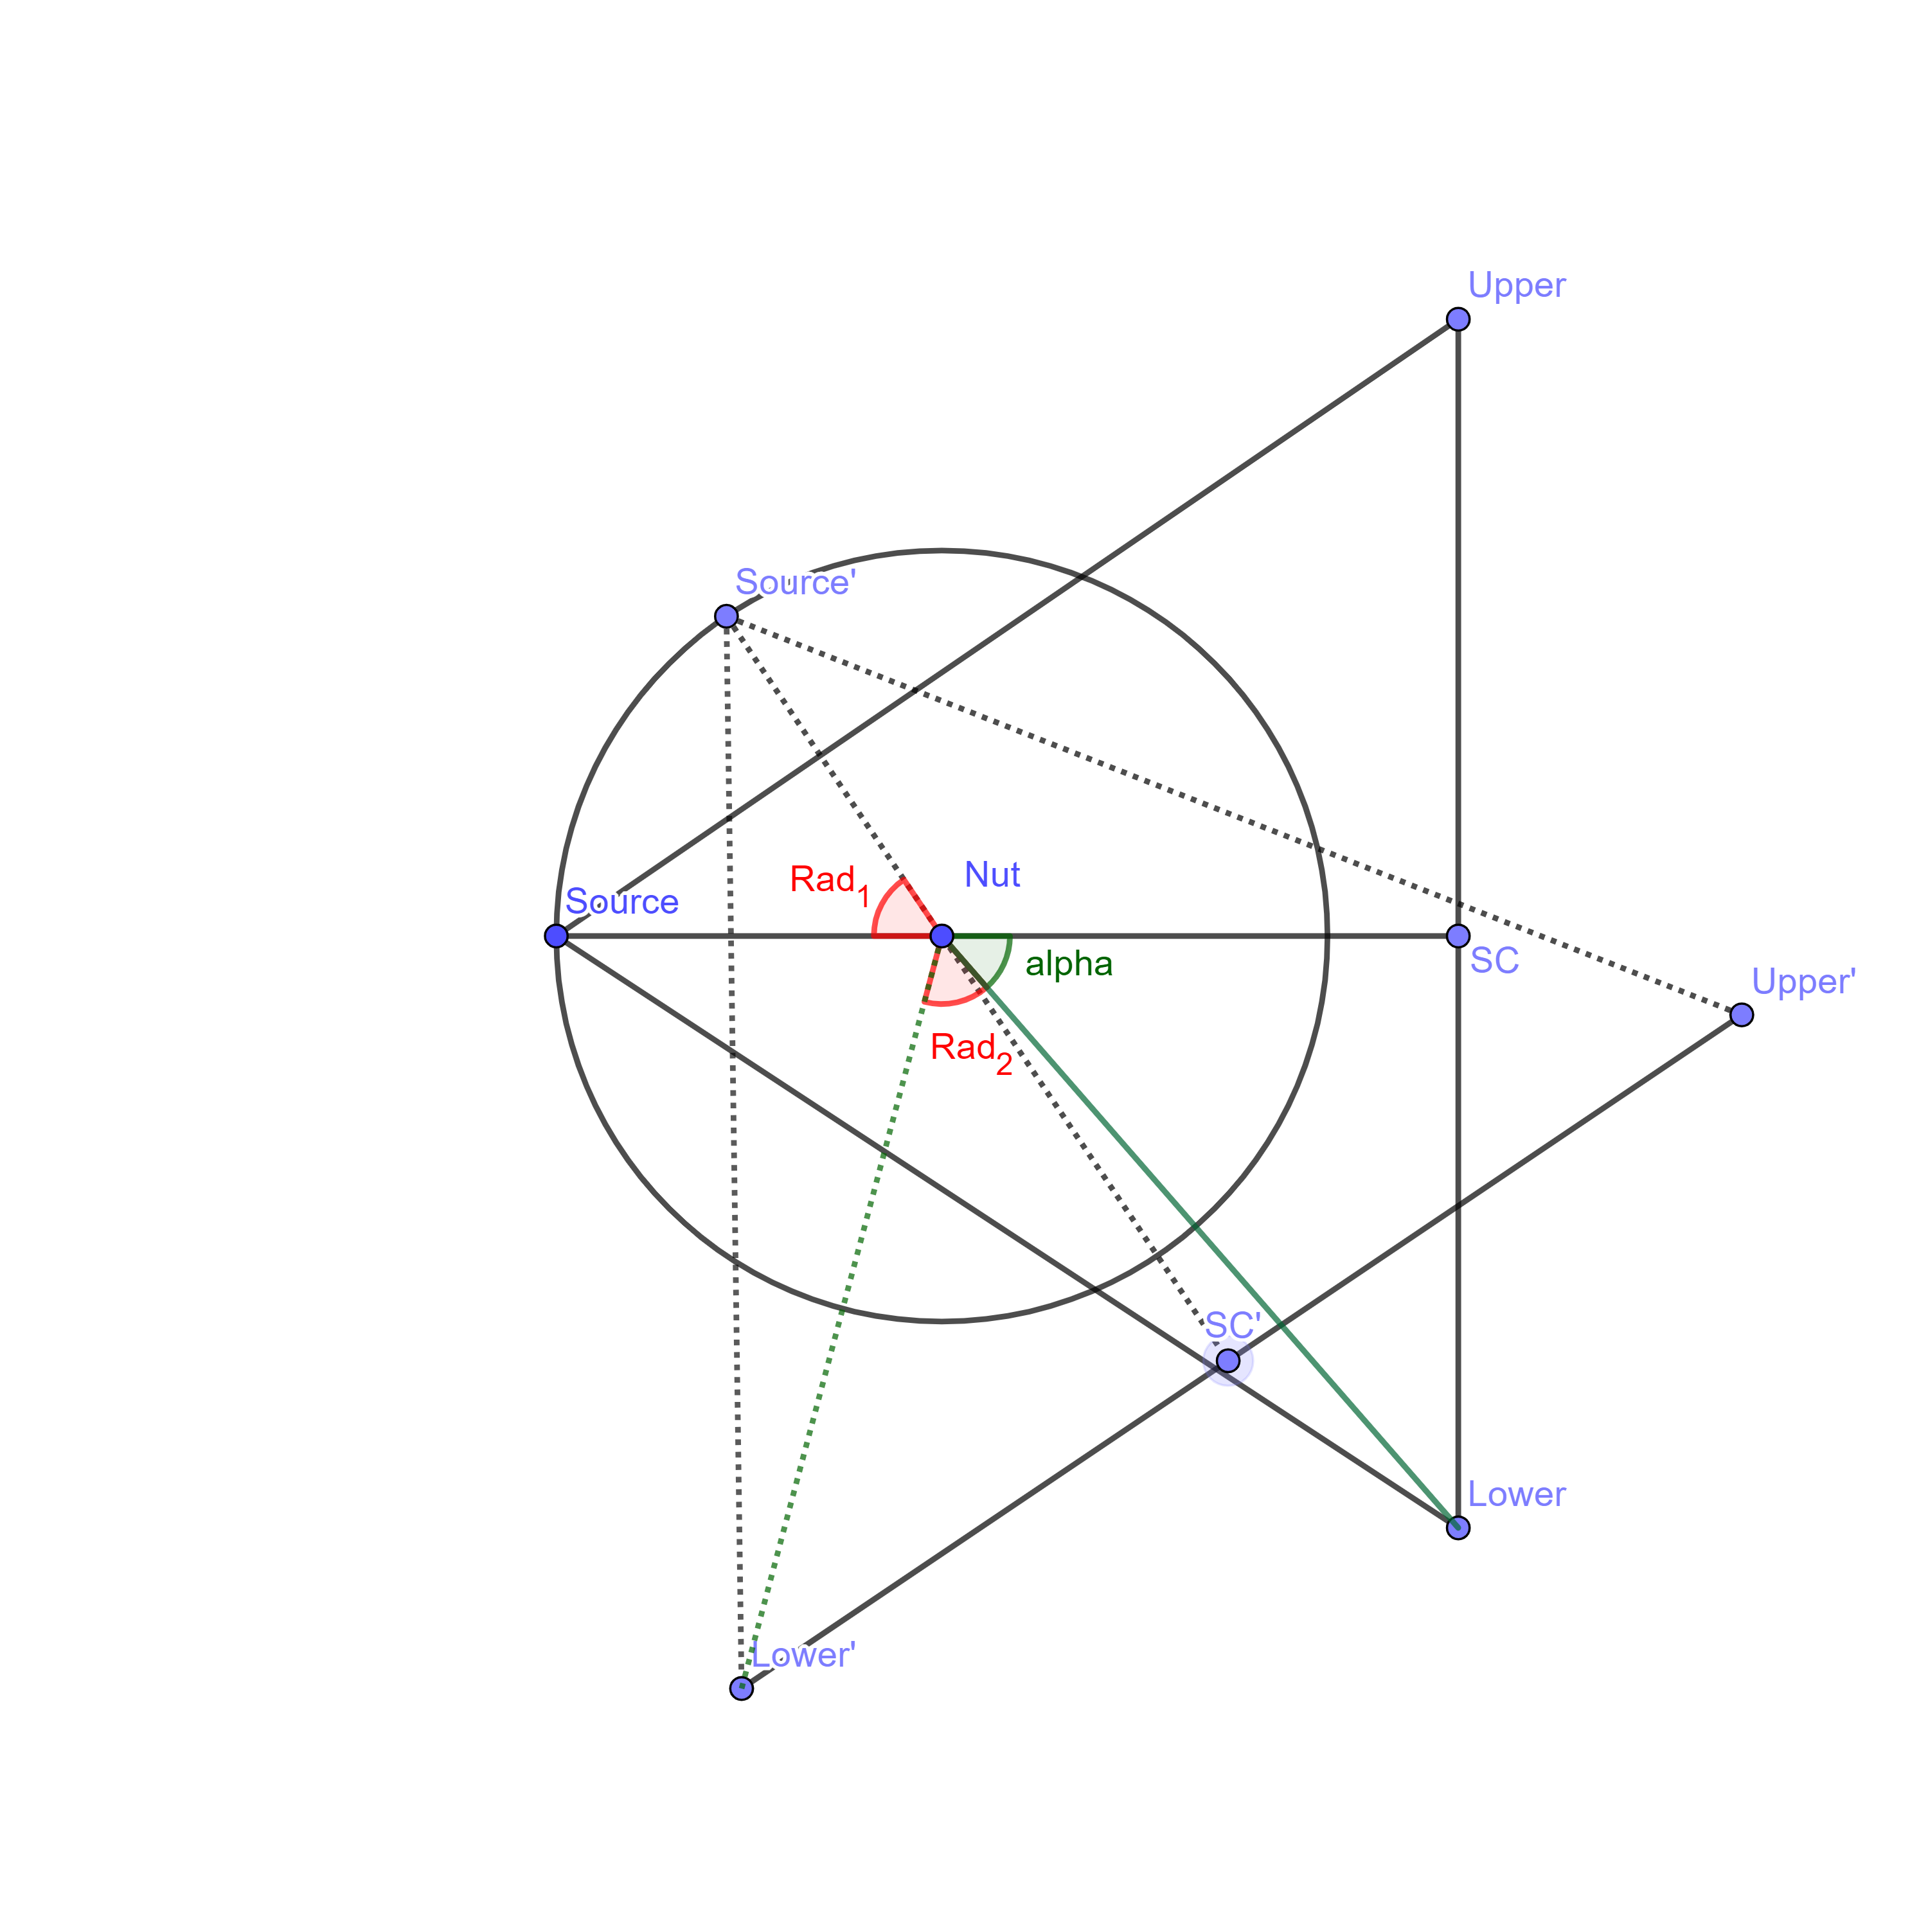
\includegraphics[width=0.4\textwidth]{k4.2/versuchsaufbau-skizze.png}
	\caption{Versuchsaufbau skizziert. \\
	$S$ steht für die Startpunkt der Strahlenquelle, $N$ ist die gescannte Walnuss, $U$ repräsentiert die obere äußere Grenzen des Detektors und $L$ respektive die Untere, $\delta$ steht für den Laufwinkel welcher in 3° Schritten erhöht wird, $\alpha$ für den Winkel zwischen X-Achse und $L$. $C$ ist der Mittelpunkt des Detektors.
	}
	\label{k4.2.fig.skizze}
\end{figure}

Anstelle einer Drehung der Nuss gegen den Uhrzeigersinn betrachten wir, äquivalent dazu, eine kreisförmigen Rotation des Detektors (Screen) und der Strahlungsquelle (S) um die Walnuss (N) (siehe \cref{k4.2.fig.skizze}). Es bieten sich Polarkoordinaten an, um die Position der Quelle und des Detektors relativ zu Walnuss zu bestimmen, jedoch müssen alle Punkte für die Weiterverarbeitung im kartesischen Koordinatensystem angegeben. Da die Winkel und Abstandsmaße in Bezug auf die Walnuss angegeben sind, wird diese als Koordinatenursprung definiert. Ausgehend davon wird die Quelle zunächst an die Stelle $\begin{pmatrix}-110\\ 0 \end{pmatrix}$   gelegt (siehe \cref{k4.2.fig.geo}, \cref{k4.2.fig.skizze}). Dadurch wird die Startposition des Detektors festgelegt, der durch seinen Anfang ($U$) an Stelle $\begin{pmatrix}190\\ 57.4 \end{pmatrix}$ und seinen Endpunkt ($L$) an Stelle $\begin{pmatrix}190\\ -57.4 \end{pmatrix}$ bestimmt wird. 
$S‘$ entspricht $S$ nach einer Drehung der Quelle und des Detektors um den Winkel $\delta$. Der Abstand zwischen $S‘$ und $\mathrm{N}$ ist dabei immer 110 mm. Der Versuchsaufbau kann somit als Einheitskreis mit Mittelpunkt $N$ interpretiert werden, der um den Faktor 110 mm gestreckt wurde. Dadurch ist im kartesischen Koordinatensystem die horizontale Koordinaten-Komponente von $S‘$ gleich $\cos(\delta) * 110\text{ mm}$ und die vertikale Komponente gleich $\sin(\delta) * 110\text{ mm}$.
Der Winkel $\sphericalangle U-N-L$ hat eine Größe von etwa 34°, somit hat der Winkel $\alpha = \sphericalangle L-N-C$ eine Größe von 17°. Der Abstand von $N$ zu $L$ kann mithilfe des Satzes von Pythagoras berechnet werden $d = \sqrt{(300\text{ mm} - 110\text{ mm})^2+(114.8\text{ mm}/2)^2} = 198.48\text{ mm}$.
Der Winkel $\alpha$ addiert mit $\delta$ ergibt zusammen mit der Länge $d$ die Koordinaten $L$ im Polarkoordinaten. Um $U‘$ zu berechnen muss $\alpha$ von $\delta$ subtrahiert werden. Die entsprechenden kartesischen Koordinaten erhalten wir nun auf gleiche Weise bei $S‘$. Die restlichen 328 Pixelpositionen des Detektors sind gleichmäßige auf der Verbindumgsstecke zwischen $U$ und $L$ verteilt.
Mit den erhaltenen Start- und Endpunkten können die Helligkeitswerte zum Raum der Dichteverteilung zurückprojiziert werden.
Die erhaltenen Start und Endpunkte, in Kombination mit den im Datenset gelieferten Helligkeitswerten kann nun in ein vollständing rüchprojeziertes CT Schichtbild verwandelt werden.


\subsection{Rekonstruktion des Signals}
\sectionauthor{Chuyang Wang}

Das Ziel der Computertomographie ist, das Signal aus den gemessenen Daten zu berechnen. Mit Bayes' Formel aus \cref{k4.2.bayes} kann man den gesuchten Posterior $P(s|d)$ mit der Likelihood $P(d|s)$ und Prior $P(s)$ wie folgt konstruieren:

\begin{equation}
  P(s|d) \propto P(d|s)P(s)\ .
\end{equation}

Für die Likelihood gilt:

\begin{equation}
  \begin{aligned}
    && P(d|s) &= \int P(d,n|s) \,dn  \\
    &&  &= \int P(d|s,n) P(n|s) \,dn \\
    && &= \int P(d|s,n) P(n) \,dn \ .
  \end{aligned}
\end{equation}

Es gilt außerdem das Datenmodell \cref{k4.2.ct.3d.datamodel}. Da bei $P(d|s,n)$ $s$ und $n$ bekannt sind, ist auch $d$ fest. Eine empirische Analyse der Daten hat gezeigt, dass das Rauschen $P(n) = \mathcal{G}(n,N)$ normalverteilt ist. Für normal verteiltes Rauschen lässt sich zeigen, dass folgende Gleichung gilt:

% delta Distribution
\begin{equation}
  \begin{aligned}
    &\Rightarrow& P(d|s) &= P_n(n-(d-Rs)) \\ 
    && &= \mathcal{G}(d-Rs,N) \ .
  \end{aligned}
\end{equation}

Die Daten $d$ wurden im Experiment gemessen (vgl. \cref{k4.2.ct.walnuss}). Die Response $R$ beschreibt das Experiment (vgl. \cref{k4.2.ct.resp}) und kann vorberechnet werden. Um den Posterior zu bestimmen, muss man die Annahmen für das Signal $s$ formulieren. Man wählt dafür ein hierarchisches Modell (vgl. \cref{k4.2.hiera}). Dabei nutzt man aus, dass $s$ positiv sein muss. Also kann man $s$ mit einer Log-Normalverteilung beschreiben. 

Um den Posterior $P(s|d) = \frac{P(d|s)P(s)}{P(d)}$ zu berechnen, benötigt man auch die Evidenz als Normierungsfaktor. Diese ist jedoch computational zu teuer. Man nutzt die Kullback-Leibler-Divergenz (vgl. \cref{k4.2.kldiv}), um den Posterior mit $P_a$ anzunähern $\mathrm{KL}(P_a,P)$. 


\subsection{Endergebnis}

Implementiert man das obige Verfahren, so erhält man am Ende eine approximative Wahrscheinlichkeitsverteilung für das Signal $P(s|d)$ mit gegebenen Daten $d$. Die \cref{k4.2.fig.ct.mean} zeigt den Erwartungswert über mehrere Stichproben der approximativen Verteilung. An der Standardabweichung \cref{k4.2.fig.ct.std} erkennt man, dass die absolute Unsicherheit an den Stellen der Walnuss höher ist, an denen besonders viel Walnuss-Masse liegt. 

\begin{figure}
  \centering
  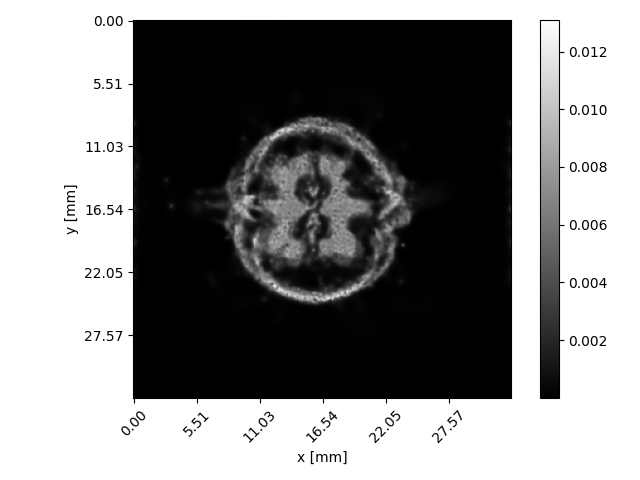
\includegraphics[width=0.6\textwidth]{k4.2/ct-walnuss-mean.png}
  \caption{Erwartungswert des Posteriors.}
  \label{k4.2.fig.ct.mean}
\end{figure}

\begin{figure}
  \centering
  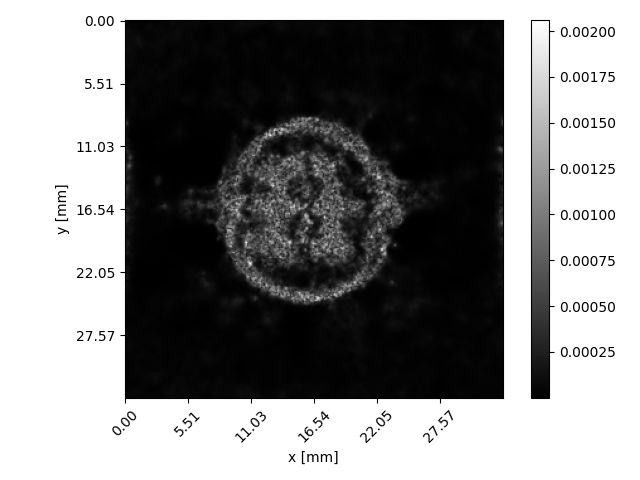
\includegraphics[width=0.6\textwidth]{k4.2/ct-walnuss-std.png}
  \caption{Standardabweichung des Posteriors.}
  \label{k4.2.fig.ct.std}
\end{figure}

An manchen Stellen wie z.B. $(10|17)$ und $(22|20)$ der \cref{k4.2.fig.ct.mean} sind unscharfe Kanten sowie teilweise Rauschen zu erkennen. Diese Fehler bei dem Modell könnten daran liegen, dass das Optimum von der Kullback-Leibler-Divergenz nur annäherungsweise erreicht ist. Darüber hinaus ist das Modell eventuell zu stark vereinfachend für die Beschreibung der Walnuss. 


\section{Posterior}

Informationstheorie mag zwar ein äußerst herausforderndes Fachgebiet sein, mit genügend Kaffee und geduldigen Erklärungen kann jedoch alles verstanden werden. Die Begeisterung für die Themen und Methoden, welche in verschiedensten naturwissenschaftlichen Bereichen Anwendung finden, werden wir noch lange in uns tragen. Von Bayes’scher Statistik bis zu Radioastronomie haben unsere Kursleiter Gordian und Philipp uns mit viel Spaß unterschiedlichste Themen nähergebracht. Und auch außerhalb der Kurszeit wurde es nicht langweilig. Der Dank für diese Akademie gilt den Kursleitenden, der Akademieleitung, sowie allen anderen Beteiligten, die mitverantwortlich für die Gestaltung dieser großartigen Zeit waren. Durch die Akademie sind wir alle zu einer Gemeinschaft geworden, in der wir aufgrund unserer Unterschiede alle voneinander lernen und uns weiterentwickeln konnten. Dies wurde durch die allgemeine Freundlichkeit und Offenheit ermöglicht. In den KüAs gaben Teilnehmer:innen ihre Begeisterung für verschiedenste Hobbys weiter, vermittelten Fähigkeiten und gaben Denkanstöße in viele Richtungen. Durch die vielfältigen Begegnungen wird uns die Zeit auf der Akademie noch lange in Erinnerung bleiben.


% Bibliography
\printbibliography{}
\end{document}
